\documentclass[10pt]{memoir}
\setstocksize{220mm}{155mm} 	        
\settrimmedsize{220mm}{155mm}{*}	
\settypeblocksize{170mm}{116mm}{*}	
\setlrmargins{18mm}{*}{*}
\setulmargins{*}{*}{1.2}
%\setlength{\headheight}{5pt}%
\checkandfixthelayout[lines]
\linespread{1.16}
\flushbottom

%%% Hyphenation settings
\usepackage[htt]{hyphenat}
\hyphenation{he-lio-trope opos-sum}
\tracingparagraphs=1
%Hyphenation in Devanāgarī of the edition still missing? Probably this needs to be modified in babel-iast package? 

%%% babel
\usepackage[english]{babel}
\usepackage{babel-iast/babel-iast}

\babelfont[iast]{rm}[Renderer=Harfbuzz, Scale=1.3]{AdishilaSan}%AdishilaSan}
\babelfont[english]{rm}{Adobe Text Pro}

%%% more functionality
\PassOptionsToPackage{hyphens}{url}
\usepackage{hyperref}
\usepackage{pdflscape}
\usepackage{cleveref}
\usepackage{url}
\usepackage{cleveref}
\usepackage{microtype}
\usepackage{lineno}

%\usepackage{bigfoot}
%%% more functions
\usepackage[dvipsnames]{xcolor}
%\usepackage[para,perpage]{footmisc}

%%%für den Counter von Kapiteln und Sätzen! 
\newcommand{\uproman}[1]{\uppercase\expandafter{\romannumeral#1}}
\newcommand{\lowroman}[1]{\romannumeral#1\relax}

\makeindex
\newfontfamily\sanskritfont[Script=Devanagari,Mapping=RomDev,Scale=1.1]{Sanskrit2003}
\usepackage{pifont,fourier-orns,lettrine,psvectorian,paralist,enumitem,pdfpages,wrapfig,tabulary,lettrine,longtable}
\setlist[enumerate]{itemsep=0mm}
\usepackage[autostyle]{csquotes}
\usepackage[defaultlines=2,all]{nowidow}
\usepackage{ellipsis,adforn,booktabs,longtable,url,tikz}
\lineskiplimit=-3pt          

\makechapterstyle{IeT}{%
  \chapterstyle{default}
  \renewcommand*{\printchapternonum}{\centering}
  \renewcommand*{\clearforchapter}{\cleartorecto} 
  \aliaspagestyle{chapter}{empty}}
\chapterstyle{IeT}
\setsecnumdepth{none}  \openright  \nouppercaseheads
\settocdepth{subsubsection}

%%%% test better pagebreaks
%\def\fussy{%
%  \emergencystretch\z@
%  \tolerance 200%
%  \hfuzz .1\p@
%  \vfuzz\hfuzz}

%\interfootnotelinepenalty=10000\relax

%\usepackage[maxfloats=256]{morefloats}

%\maxdeadcycles=500

%raggedbottomsectiontrue
%%\checkandfixthelayout


%%%%%%%  biblatex
%\newcommand{\noun}[1]{\textsc{#1}}    %  philosophy-verbose
\usepackage[backend=biber, sorting=nyt, style=verbose]{biblatex} %%%%ORIGINAL TiE
\renewcommand*{\mkbibnamefamily}[1]{\textsc{#1}}


\DeclareFieldFormat{url}{%
  \mkbibacro{URL}\addcolon\space
  \href{#1}{\nolinkurl{\thefield{urlraw}}}}

\DeclareFieldFormat{citeurl}{%
  \href{#1}{\nolinkurl{\thefield{urlraw}}}} 


\DeclareFieldFormat{postnote}{#1}
\renewcommand{\postnotedelim}{, }
\addbibresource{bindu.bib}

%%% ekdosis
\usepackage[teiexport=tidy,parnotes=true]{ekdosis}% =tidy cleans up HTML and XML documents by fixing markup errors and upgrading legacy code to modern standards. parnotes=footnotes below or above critical apparatus

\SetLineation{lineation=page, modulo} %lineation=page sets thenumbering to start afresh at the top of each page. =modulo makes every fifth line numbered. {lineation=page} makes every line numbered! 

\renewcommand{\linenumberfont}{\selectlanguage{english}\footnotesize} %sets language of lines to English

\SetTEIxmlExport{autopar=false} %autopar=falseinstructs ekdosis to ignore blank lines in the.tex sourcefile as markers for paragraph boundaries. As a result, each paragraph of the edition must be found within an environment associated with the xml <p> element

\SetHooks{
  lemmastyle=\bfseries,
  %refnumstyle=\selectlanguage{english}\bfseries,
  refnumstyle=\selectlanguage{english}\color{blue}\bfseries,
  appheight=0.8\textheight,
}

\newif\ifinapparatus
\DeclareApparatus{source}[
%bhook=\inapparatustrue,
lang=english,
notelang=english,
% bhook=\selectlanguage{english},
bhook=\selectlanguage{english}\textbf{Sources:},%
%maxentries=4, 
%ehook=.]
%sep={] },
%nosep,
]

\newif\ifinapparatus
\DeclareApparatus{testium}[
%bhook=\inapparatustrue,
lang=english,
notelang=english,
% bhook=\selectlanguage{english},
bhook=\selectlanguage{english}\textbf{Testimonia:},
%maxentries=4, 
%ehook=.]
%nosep, 
]

% Declare \ifinapparatus and set \inapparatustrue at the beginning of
% the apparatus criticus block. Also set the language.  
\newif\ifinapparatus
  \DeclareApparatus{default}[
  %bhook=\inapparatustrue, 
  lang=english,
  %maxentries=33,
  %bhook=\selectlanguage{english},
  sep = {] },
  delim=\hskip 0.75em,
  rule=\rule{0.7in}{0.4pt},
]

\newif\ifinapparatus
\DeclareApparatus{philcomm}[
%bhook=\inapparatustrue,
lang=english,
notelang=english,
bhook=\selectlanguage{english}\textbf{Philological Commentary:},
%bhook=\selectlanguage{english},
sep={: },
]

\ekdsetup{
showpagebreaks,
spbmk = \textcolor{blue}{spb},
hpbmk = \textcolor{red}{hpb}
}

%\usepackage{fnpos}
%\makeFNmid
%\makeFNbottom
\usepackage[bottom]{footmisc}
%%%%%%%%%%%%%%%%%%%%%%%%%%%
\makeatletter
\def\blfootnote{\gdef\@thefnmark{}\@footnotetext}
\makeatother
%%%%%%%%%%%%%%%%%%%%%%%%%


% Macros and Definitions for the Print of Sigla
\def\acpc#1#2#3{{#1}\rlap{\textrm{\textsuperscript{#3}}}\textsubscript{\textrm{#2}}\space}
\def\sigl#1#2{{{#1}}\textsubscript{\textrm{#2}}}
\def\None{{\sigl{N}{1}}} \def\Noneac{\acpc{N}{1}{ac}\,} \def\Nonepc{\acpc{N}{1}{pc}\,}
\def\Ntwo{{\sigl{N}{2}}} \def\Noneac{\acpc{N}{2}{ac}\,} \def\Nonepc{\acpc{N}{2}{pc}\,}
\def\Done{{\sigl{D}{1}}} \def\Doneac{\acpc{D}{1}{ac}\,} \def\Donepc{\acpc{D}{1}{pc}\,}
\def\Dtwo{{\sigl{D}{2}}} \def\Dtwoac{\acpc{D}{2}{ac}\,} \def\Dtwopc{\acpc{D}{2}{pc}\,}
\def\Uone{{\sigl{U}{1}}} \def\Uoneac{\acpc{U}{1}{ac}\,} \def\Uonepc{\acpc{U}{1}{pc}\,}                 
\def\Utwo{{\sigl{U}{2}}} \def\Utwoac{\acpc{U}{2}{ac}\,} \def\Utwopc{\acpc{U}{2}{pc}\,}

%%%%%%%%%%%%%% Tattvabinduyoga - List of Witnesses   %%%%%%%%%%%%%%%%%%%
\DeclareWitness{ceteri}{\selectlanguage{english}cett.}{ceteri}[]   
\DeclareWitness{E}{\selectlanguage{english}E}{Printed Edition}[]    
\DeclareWitness{P}{\selectlanguage{english}P}{Pune BORI 664}[]  
\DeclareWitness{B}{\selectlanguage{english}B}{Bodleian 485}[]       
\DeclareWitness{N1}{\selectlanguage{english}N\textsubscript{1}}{NGMPP 38/31}[]
\DeclareWitness{N2}{\selectlanguage{english}N\textsubscript{2}}{NGMPP B 38/35}[]
\DeclareWitness{L}{\selectlanguage{english}L}{LALCHAND 5876}[]  
\DeclareWitness{D}{\selectlanguage{english}D}{IGNCA 30019}[] 
%\DeclareWitness{D2}{\selectlanguage{english}D\textsubscript{2}}{IGNCA 30020}[]  
\DeclareWitness{U1}{\selectlanguage{english}U\textsubscript{1}}{SORI 1574}[] 
\DeclareWitness{U2}{\selectlanguage{english}U\textsubscript{2}}{SORI 6082}[]
%%%%%%%%%%%%%% Tattvabinduyoga - Groups of Witnesses   %%%%%%%%%%%%%%%%%%%
\DeclareWitness{X}{\selectlanguage{english}\alpha}{Alpha Group: D,N1,N2,U1}[]
\DeclareWitness{Y}{\selectlanguage{english}\beta}{Beta Group: B,E,L,P,U2}[]
%%%%%%%%%%%%% Testimonia
\DeclareWitness{Ysv}{\selectlanguage{english}Ysv}{Yogasvarodaya}[] %%%add infos!  

%%%%%%%%%%%%%%%%%%%%%%%%%%%%%%%%%%%%%%%%%%%
% Macro for Editing Abbrevs.
\def\om{\textrm{\footnotesize \textit{om.}\ }} %prints om. for omitted in apparatus
\def\korr{\textrm{\footnotesize \textit{em.}\ }} %prints em. for emended in apparatus
\def\conj{\textrm{\footnotesize \textit{conj.}\ }} %prints conj. for conjectured in apparatus

% \supplied{text} EDITORIAL ADDITION -> Within \lem oder \rdg
% \surplus{text} EDITORIAL DELETION -> Within \lem oder \rdg
% \sic{text} CRUX
% \gap{text} LACUNAE -> [reason=??, unit=??, quantity=??, extent=??]


%%%%%%%%%%%%%%%%%%%%%%%%%%%%%%%%%%%%%%%%%%% All macros of this list can be used in 
% Macro for Editing Abbrevs.
\def\eyeskip{\textrm{{ab.\,oc. }}}
\def\aberratio{\textrm{{ab.\,oc. }}}
\def\ad{\textrm{{ad}}}
\def\add{\textrm{{add.\ }}}
\def\ann{\textrm{{ann.\ }}}
\def\ante{\textrm{{ante }}} 
\def\post{\textrm{{post }}}
%\def\ceteri{cett.\,}                   
\def\codd{\textrm{{codd.\ }}}

\def\coni{\textrm{{coni.\ }}}
\def\contin{\textrm{{contin.\ }}}
\def\corr{\textrm{{corr.\ }}}
\def\del{\textrm{{del.\ }}}
\def\dub{\textrm{{ dub.\ }}}

\def\expl{\textrm{{explic.\ }}} 
\def\explica t{\textrm{{explic.\ }}}
\def\fol{\textrm{{fol.\ }}}
\def\foll{\textrm{{foll.\ }}}
\def\gloss{\textrm{{glossa ad }}}
\def\ins{\textrm{{ins.\ }}}      
\def\inseruit{\textrm{{ins.\ }}} 
\def\im{{\kern-.7pt\lower-1ex\hbox{\textrm{\tiny{\emph{i.m.}}}\kern0pt}}} %\textrm{\scriptsize{i.m.\ }}}      
\def\inmargine{{\kern-.7pt\lower-.7ex\hbox{\textrm{\tiny{\emph{i.m.}}}\kern0pt}}}%\textrm{\scriptsize{i.m.\ }}}      
\def\intextu{{\kern-.7pt\lower-.95ex\hbox{\textrm{\tiny{\emph{i.t.}}}\kern0pt}}}%\textrm{\scriptsize{i.t.\ }}}           
\def\indist{\textrm{{indis.\ }}}  
\def\indis{\textrm{{indis.\ }}}
\def\iteravit{\textrm{{iter.\ }}} 
\def\iter{\textrm{{iter.\ }}}
\def\lectio{\textrm{{lect.\ }}}   
\def\lec{\textrm{{lect.\ }}}
\def\leginequit{\textrm{{l.n. }}} 
\def\legn{\textrm{{l.n. }}}
\def\illeg{\textrm{{l.n. }}}

\def\primman{\textrm{{pr.m.}}}
\def\prob{\textrm{{prob.}}}
\def\rep{\textrm{{repetitio }}}
\def\secundamanu{\textrm{\scriptsize{s.m.}}}            \def\secm{{\kern-.6pt\lower-.91ex\hbox{\textrm{\tiny{\emph{s.m.}}}\kern0pt}}}%   \textrm{\scriptsize{s.m.}}}
\def\sequentia{\textrm{{seq.\,inv.\ }}}  
\def\seqinv{\textrm{{seq.\,inv.\ }}}
\def\order{\textrm{{seq.\,inv.\ }}}
\def\supralineam{{\kern-.7pt\lower-.91ex\hbox{\textrm{\tiny{\emph{s.l.}}}\kern0pt}}} %\textrm{\scriptsize{s.l.}}}
\def\interlineam{{\kern-.7pt\lower-.91ex\hbox{\textrm{\tiny{\emph{s.l.}}}\kern0pt}}}   %\textrm{\scriptsize{s.l.}}}
\def\vl{\textrm{v.l.}}   \def\varlec{\textrm{v.l.}} \def\varialectio{\textrm{v.l.}}
\def\vide{\textrm{{cf.\ }}}
\def\cf{\textrm{{cf.\ }}} 
\def\videtur{\textrm{{vid.\,ut}}}
\def\crux{\textup{[\ldots]} }
\def\cruxx{\textup{[\ldots]}}
\def\unm{\textit{unm.}}
%%%%%%%%%%%%%%%%%%%%%%%%%%%%%%%%%%%%

% List of Scholars
\DeclareScholar{ego}{ego}[
forename=Nils Jacob,
surname=Liersch]

% Persons:14\DeclareScholar{ego}{ego}[15forename=Robert,16surname=Alessi]17% Useful shorthands:18\DeclareShorthand{codd}{codd.}{V,I,R,H}19\DeclareShorthand{edd}{edd.}{Lit,Erm,Sm}20\DeclareShorthand{egoscr}{\emph{scripsi}}{ego}

%Useful shorthands:
%\DeclareShorthand{codd}{codd.}{V,I,R,H}
%\DeclareShorthand{edd}{edd.}{Lit,Erm,Sm}
\DeclareShorthand{egoscr}{em.}{ego}
\DeclareShorthand{egoscrconj}{conj.}{ego}
\DeclareShorthand{egomute}{\unskip}{ego}

\usepackage{xparse}

\NewDocumentEnvironment{tlg}{O{}O{}}{\setlength{\leftskip}{0pt}\vspace{-1ex}\begin{quotation}}{\hfill #1\ \vspace{-1ex}\end{quotation}\vspace{-1ex}} %verse environment
%\NewDocumentEnvironment{tlg}{O{}O{}}{\begin{verse}}{॥#1\hskip-4pt ॥\\ \end{verse}}
\NewDocumentCommand{\tl}{m}{{\selectlanguage{iast} #1}}

\NewDocumentCommand{\extra}{m}{{\textcolor{gray}{#1}}} %command for additions to U2
\NewDocumentCommand{\crazy}{m}{{\textcolor{red}{#1}}} %totally corrupted passage
\NewDocumentCommand{\coro}{m}{{\textcolor{violet}{#1}}} %colour for sentence counter! 

\NewDocumentEnvironment{prose}{O{}}{\begin{otherlanguage}{iast}}{\end{otherlanguage}}
% \NewDocumentEnvironment{padd}{O{}}{\begin{otherlanguage}{iast}}{\end{otherlanguage}}
\NewDocumentEnvironment{tlate}{O{}}
%\NewDocumentEnvironment{tadd}{O{}}

%Define two commands: \skp ("sanskrit plus"), to be ignored by TeX in
%the edition text, but processed in the TEI output. Conversely, \skm
%("sanskrit minus") is to be processed in the edition text, but
%ignored if found in the apparatus criticus and in the TEI output:

\NewDocumentCommand{\skp}{m}{}
\TeXtoTEIPat{\skp {#1}}{#1}

%\NewDocumentCommand{\skpp}{m}{}
%\TeXtoTEIPat{\skpp {#1}}{#1}

\NewDocumentCommand{\skm}{m}{\unless\ifinapparatus#1-\fi}
\TeXtoTEIPat{\skm {#1}}{}

% \NewDocumentCommand{\dd}{}{/\hskip-4pt/}
\NewDocumentCommand{\dd}{}{\mbox{/\hskip-4pt/}}
\TeXtoTEIPat{\dd {}}{//}


%%% modify environments and commands
%%% TEI mapping
\TeXtoTEIPat{\begin {tlg}}{<lg>} %lg=(Group of verse (s)) contains one or more verses or lines of verse that together form a formal unit (e.g. stanza, chorus).
\TeXtoTEIPat{\end {tlg}}{</lg>}

\TeXtoTEIPat{\begin {prose}}{<p>}
\TeXtoTEIPat{\end {prose}}{</p>}

\TeXtoTEIPat{\begin {tlate}}{<p>}
\TeXtoTEIPat{\end {tlate}}{</p>}

\TeXtoTEIPat{\\}{}
\TeXtoTEIPat{\linebreak}{<br/>}
\TeXtoTEIPat{\noindent}{}
%\TeXtoTEI{tl}{l}
\TeXtoTEI{emph}{hi}
\TeXtoTEI{bigskip}{}
\TeXtoTEI{None}{N1}
\TeXtoTEI{Ntwo}{N2}
\TeXtoTEI{Done}{D1}
\TeXtoTEI{Dtwo}{D2}
\TeXtoTEI{Uone}{U1}
\TeXtoTEI{Utwo}{U2}
%\TeXtoTEIPat{/}{ |}
%\TeXtoTEI{//}{ ||}
\TeXtoTEIPat{\korr}{em. }
\TeXtoTEIPat{\conj}{conj.}
\TeXtoTEIPat{\om}{om.}
\TeXtoTEIPat{english}{}
\TeXtoTEIPat{\hskip}{}
\TeXtoTEIPat{\hskip-4pt}{}
\TeXtoTEIPat{\hskip-2pt}{}
\TeXtoTEIPat{-}{ }
\TeXtoTEIPat{4pt}{}
\TeXtoTEIPat{2pt}{}
\TeXtoTEIPat{\textcolor {#1}{#2}}{<hi rend="#1">#2</hi>} 

% Nullify \selectlanguage in TEI as it has been used in
% \DeclareWitness but should be ignored in TEI.
\TeXtoTEI{selectlanguage}{}



\FormatDiv{1}{\begin{center}\Large}{\end{center}}
\FormatDiv{2}{\begin{center}\small}{\end{center}}
\FormatDiv{3}{\bfseries}{.}
\title{Yogatattvabindu of Rāmacandra\\ A Critical Edition and Annotated Translation}
\date{\today}

\parindent=15pt
\begin{document}

%Zitiermöglichkeiten:
%\footcite[See][p.\,1]{goldstein01:_tibet_englis_diction_moder_tibet}
%\footnote{\cite{goldstein01:_tibet_englis_diction_moder_tibet}.}

\frontmatter
\thispagestyle{empty}
\begin{center}
  {\Large \emph{The Yogatattvabindu}}\\[3mm]
\end{center}



\newpage

\

\thispagestyle{empty}



\normalsize


\newpage


\begin{center}
\thispagestyle{empty}

\

\vskip 2mm

\begin{otherlanguage}{iast}
\LARGE \sanskritfont{Yogatattvabindu}
\end{otherlanguage}

\vskip .4cm

\Huge Yogatattvabindu \\[7mm]
\Large Critical Edition\\
with annotated Translation


\large

\vspace{3cm}

Von

Nils Jacob Liersch
\small
\vfill

\vfill

Indica et Tibetica Verlag \\ % $\cdot$ 
Marburg 2024

\vskip 6mm

\end{center}

\newpage
\newpage \ \thispagestyle{empty}
\small  \

\noindent

\
\vfill


\small
\noindent \textbf{Bibliographische Information Der Deutschen Bibliothek}

\noindent
Die Deutsche Bibliothek verzeichnet diese Publikation in der Deutschen Nationalbibliographie;
detaillierte bibliographische Informationen sind im Internet über http://dnb.ddb.de abrufbar.

\noindent
\textbf{Bibliographic information published by Die Deutschen Bibliothek}

\noindent
Die Deutsche Bibliothek lists this publication in the Deutsche Nationalbibliographie; detailed
bibliographic data is available in the Internet at http://dnb.ddb.de.  


\vskip 1cm

\noindent
\copyright\ Indica et Tibetica Verlag, Marburg 2024

\medskip

\noindent
Alle Rechte vorbehalten / All rights reserved

\medskip

\noindent
Ohne ausdrückliche Genehmigung des Verlages ist es nicht gestattet, das Werk oder einzelne Teile
daraus nachzudrucken, zu vervielfältigen oder auf Datenträger zu speichern.

\smallskip

\noindent
Apart from any fair dealing for the purpose of private study, research, criticism or review, no
part of this book may be reproduced or translated in any form, by print, photo form, microfilm, or
any other means without written permission. Enquiries should be made to the publishers.

\bigskip

\noindent
Satz: \ \ Nils Jacob Liersch \\
Herstellung: \ \ BoD – Books on Demand GmbH, Norderstedt  \\

\bigskip

\noindent
%\ISBN     

\normalsize

\newpage

%\maketitle
\clearpage
\tableofcontents
\addtocounter{page}{-1}
\thispagestyle{empty}
\clearpage


\mainmatter

\chapter{Conventions in the Critical Apparatus}
\section{Sigla in the Critical Apparatus}

\begin{itemize}
\item E : Printed Edition
\item P : Pune BORI 664
\item L : Lalchand Research Library LRL5876
\item B : Bodleian Oxford D 4587
‚\item \None : NGMPP B 38-31
\item \Ntwo : NGMPP B 38-35 / A 1327-14
\item \Done : IGNCA 30019
\item \Uone : SORI 1574
\item \Utwo: SORI 6082
\end{itemize}

\chapter{Critical Edition \& Annotated Translation}
\cleardoublepage
\begin{alignment}[
  texts=edition[class="edition"];
  translation[class="translation"],
  ]
  \begin{edition}
    \begin{prose}[p57_04]
      \noindent
%\note[type=philcomm, labelb=400x, labele=_400xe, lem={taṃ sadguruṃ jānīyāt \ldots yogarahasyaṃ karttavyaṃ}]{Passage possibly authorial.}
%-----------------------------
%taṃ sadguruṃ vijānīyāt vikalpa etādaśo  yathā samudramadhye mahattaraṃ kallolāḍambaram/ prapaṃce vāsanā   tādṛśī yathodakamadhye mahattaraṃgāḥ/    \E
%taṃ sadguruṃ jānīyāt   vikalpa etādṛśo  yathā samudramadhye mahattara--kallolāḍambaraṃ  prapaṃca-vāsanā  etādṛśī yathodakamadhye mahattarati        \P
%taṃ sadguruṃ jānīyāt   vikalpa etādṛśo  yathā samudramadhye mahattara--kallolāḍambara   prapaṃca-vāsanā  etādṛśī yathodakamadhye mahattarati ....   \B
%taṃ sadguruṃ jānīyāt   vikalpa etādṛśo  yathā samudramadhye mahattara--kallolāḍambara   prapaṃca-vāsanā  etādṛśī yathodakamadhye mahattarati ....   \L
%taṃ sadguruṃ jānīyāt// vikalpa etādṛśo  yathā samudramadhye mahattara--kallolāḍambaraḥ/ prapaṃca-vāsanā  etādṛśī yathodakamadhye mahattarati        \N1
%taṃ sadguruṃ jānīyāt// vikalpa etādṛśaṃ yathā samudramadhye mahattara--kallolāḍambaraḥ  prapaṃca-vāsanā  etādṛśī yathodakamadhye mahattarati        \N2 %%S.12
%taṃ sadguruṃ jānīyāt/  vikalpa etādṛśo  yathā samudramadhye mihattara--kallolāḍambaraḥ/ prapaṃca-vāsanā  etādṛśī yathodakamadhye mahattarati        \D
%taṃ sadguruṃ jānīyāt// vikalpa etādṛśo  yathā samudramadhye mahattara--kallolāḍambaraṃ  prapaca vāsanā// etādṛśī yathodakamadhye mahattarī          \U2
%\om \U1
%-----------------------------
%E: One should know this true teacher. The changing thought is like the roar of waves within the ocean. The manifold mental imprints are like the ripples in the water...
%----------------------------30-31
taṃ sadguruṃ
\app{\lem[wit={ceteri}]{jānīyāt}
  \rdg[wit={E}]{vijānīyāt}}/
vikalpa
\app{\lem[wit={ceteri}]{etādṛśo}
  \rdg[wit={N2}]{etādṛśaṃ}}
yathā samudramadhye
\app{\lem[wit={ceteri},alt={mahattara°}]{mahattara}
  \rdg[wit={D}]{mihattara}
  \rdg[wit={E}]{mahattaraṃ}
}kallolā\app{\lem[wit={ceteri},alt={°ḍambaraḥ}]{ḍambaraḥ}
  \rdg[wit={B,L}]{°ḍambara°}
  \rdg[wit={E,P,U2}]{°ḍambaraṃ}}
\app{\lem[wit={ceteri},alt={prapañca°}]{prapañca}
  \rdg[wit={U2}]{prapaca}}vāsanā 
\app{\lem[wit={ceteri}]{etādṛśī}
  \rdg[wit={E}]{tādṛśī}}
yathodakamadhye
\app{\lem[wit={E}]{mahattaraṅgāḥ}
  \rdg[wit={U2}]{mahattarī}
  \rdg[wit={ceteri}]{mahattarati}}/ 
%----------------------------
%tādṛśasya saṃsārasāgarasya   yaḥ svavākyanāvā paraṃ pāraṃ  prāpayati/  sa sadguruḥ kathyate// \E
%tādṛśya   saṃsārā---rṇāvād   yo          nāvā paraṃ        prāpayati   sa sadguruḥ kathyate  \P
%tādṛśāt   saṃsārā---rṇavavād yau         nāvā paraṃ        prāpayati/  sa sadguruḥ kathyate// \B
%tādṛśāt   saṃsārā---rṇavād   yau         nāvā paraṃ        prāpayati   sa sadguruḥ kathyate// \L
%tādṛśāt   saṃsārāt arṇavād  yo           nāvaraṃ           prāpayati/  sa sadguruḥ kathyate// \N1 %%%S.14 Z. 3
%tādṛśāt   saṃsārāt arṇavād  yo           nāvaraṃ           prāpayati/  sa sadguruḥ kathyate// \N2
%tādṛśāt   saṃsārāt aṛṇavād   yo          nāvā paraṃ        prāpayati/     sadguruḥ kathyate/ \D
%tādṛśāt   saṃsārā---rṇavād   yo          nāvā pāraṃ pāraṃ  prāpayati// sa sadguruḥ kathyate// \U2
%\om \U1
%-----------------------------
%He who causes to navigate/convey the boat from such an ocean of Saṃsāra to the other shore is called a true teacher. 
%-----------------------------32-33
\app{\lem[wit={ceteri}]{tādṛśāt}
  \rdg[wit={E}]{tādṛśasya}}
\app{\lem[wit={P,L,U2}]{saṃsārārṇavā\skp{d-yo}}
  \rdg[wit={B}]{saṃsārārṇavavād}
  \rdg[wit={D,N1,N2}]{saṃsārāt arṇavād}
}\app{\lem[wit={ceteri},alt={yo}]{\skm{d-yo}}
  \rdg[wit={B,L}]{yau}
  \rdg[wit={E}]{yaḥ}}
\app{\lem[wit={B,L,P,D,U2}]{nāvā}
  \rdg[wit={N1,N2}]{nāvaraṃ}
  \rdg[wit={E}]{svavākyanāvā}}
\app{\lem[wit={E}]{paraṃ pāraṃ}
  \rdg[wit={U2}]{pāraṃ pāraṃ}
  \rdg[wit={B,L,P,D}]{paraṃ}
  \rdg[wit={N1,N2}]{\om}}
prāpayati/
\app{\lem[wit={ceteri}]{sa}
  \rdg[wit={D}]{\om}}
sadguruḥ kathyate/ 
%-----------------------------
%yasya puruṣasya mano  'khaṇḍe paramapade līnaṃ bhavati/ [p.81]     \E
%yasya puruṣasya mano  'khaṃḍe       pade līnaṃ bhavati/                 \P
%yasya puruṣasya manaḥ akhaṃḍe       pade līnaṃ bhavatī/ DSCN7180.JPG   \B
%yasya puruṣasya manaḥ akhaṃḍe       pade līnaṃ bhavati/                \L
%yasya puruṣasya mano   khaṃḍe   parapada-līna bhavati/                \N1
%yasya puruṣasya mano   khaṃḍe   paramada-lita bhavati/                \N2
%yasya puruṣasya mano   khaṃḍe   parapada-līnaṃ bhavati/                \D
%yasya puruṣasya mano  'khaṇḍe   parapade līnaṃ bhavati     \U2
%\om \U1
%----------------------------
%The mind of the person becomes absorbed into the indivisible supreme place.  
%-----------------------------34
yasya puruṣasya
\app{\lem[wit={ceteri}]{mano}
  \rdg[wit={B,L}]{manaḥ}
}\app{\lem[wit={ceteri}]{'khaṇḍe}
  \rdg[wit={B,L}]{akhaṃḍe}}
\app{\lem[wit={E}]{paramapade}
  \rdg[wit={D,N1}]{parapada°}
  \rdg[wit={N2}]{paramada°}
  \rdg[wit={U2}]{parapade}}
\app{\lem[wit={ceteri}]{līnaṃ}
  \rdg[wit={N1}]{°līna}
  \rdg[wit={N2}]{°lita}}
\app{\lem[wit={ceteri}]{bhavati}
  \rdg[wit={B}]{bhavatī}}/  
%-----------------------------
%yaḥ puruṣaḥ svakulaṃ     trividhāt   tāpān nivartya  parame  muktipade  rakṣati/ \E
%yaḥ puruṣaḥ svīyaṃ kulaṃ trividhāt   tapān nivartta--parama--muktipade  rakṣati \P %%%7579.jpg
%yaḥ puruṣaḥ svikulaṃ     trividhaṃ/  tāpān nivartya  para----muktipade  rakṣati/ \B
%yaḥ puruṣaḥ sviyaṃ kulaṃ trividhat   āpān nivartya   para----muktipade  rakṣati... \L
%yaḥ puruṣaḥ svīyaṃ kūlaṃ trividhāt   tāpān nivarttya parama--muktipade  rakṣati/ \N1
%yaḥ puruṣa  svīyaṃ kūlaṃ trividhāt   tāpān nivartya  paramamamuktipade  rakṣati/ \N2
%yaḥ puruṣaḥ svīyaṃ kūlaṃ trividhāt---tāpān mivarttya parama--muktipade  rakṣati/ \D
%yaḥ puruṣa  svīyaṃ kulaṃ trividhat---āpān nivartya   parama--muktipakṣe rakṣati// \U2
%\om \U1
%-----------------------------
%The person situated in the place of supreme liberation who turned away from the threefold misery (adhyātmika, adhibhautika, adhidaivika) protects the own kula (lineage? noble family? tribe?). 
%-----------------------------35
yaḥ \app{\lem[wit={ceteri}]{puruṣaḥ}
  \rdg[wit={N2,U2}]{puruṣa}}
\app{\lem[wit={ceteri}]{svīyaṃ kūlaṃ}
  \rdg[wit={B}]{svikulaṃ}
  \rdg[wit={E}]{svakulaṃ}}
\app{\lem[wit={E,D,P,N1,N2},alt={trividhāt}]{trividhā\skp{t-tā}}
  \rdg[wit={L,U2}]{trividhat}
  \rdg[wit={B}]{trividhaṃ |}
}\app{\lem[wit={ceteri},alt={tāpān}]{\skm{t-tā}pā\skp{n-ni}}
  \rdg[wit={L,U2}]{āpān}}\skm{n-ni}vartya
\app{\lem[wit={P,D,N1}]{paramamuktipade}
  \rdg[wit={E}]{parame muktipade}
  \rdg[wit={N2}]{paramamamuktipade}
  \rdg[wit={B,L}]{paramuktipade}
  \rdg[wit={U2}]{paramamuktipakṣe}} rakṣati/
%-----------------------------
%etādṛśasya puruṣasya śravaṇād   darśanāt  samagravighnā naśyanti/    \E
%etādṛśā    puruṣasya śravaṇā    darśanāt  samagravighnā naśyaṃti     \P
%etādṛśā    puruṣasya śravaṇāt   darśanāt/ samagravighnā na naśyaṃtī/ \B
%etādṛśā    puruṣasya śravaṇāt   darśanāt  samagravighnā na naśyaṃti... \L
%etādṛśa/   puruṣaṃ   śravaṇād   darśanāt  samagravighnā naśyaṃti/ \N1
%etādṛśaṃ   puruṣaṃ   śravaṇād   darśanāt  samagravighnā naśyaṃti/ \N2
%etādṛśa----puruṣaṃ   śravaṇād   darśanāt  samagravighnā naśyaṃti/ \D
%etādṛśaṃ   puruṣaṃ   śravaṇād   darśanāt  samagraviśvaś ca vaśāṃ? bhavati \U1
%etādṛśa    puruṣasya śravaṇāt// darśanāt  samagravighna naśyaṃti//    \U2
%-----------------------------
%From hearing [or] from seeing about such a person all obstacles are destroyed. 
%-----------------------------36
\note[type=philcomm, labelb=417, lem={etādṛśaṃ \ldots naśyanti}]{Textual evidence of \getsiglum{U1} resumes from this sentence onwards.}
\app{\lem[wit={ceteri}]{etādṛśaṃ}
  \rdg[wit={D,U2}]{etādṛśa}
  \rdg[wit={N1}]{etādṛśa |}
  \rdg[wit={B,L,P}]{etādṛśā}
  \rdg[wit={E}]{etādṛśasya}}
\app{\lem[wit={X}]{puruṣaṃ}
  \rdg[wit={Y}]{puruṣasya}}
\app{\lem[wit={ceteri},alt={śravaṇād}]{śravaṇā\skp{d-da}}
  \rdg[wit={B,L}]{śravaṇāt}
  \rdg[wit={U2}]{śravaṇāt ||}
  \rdg[wit={P}]{śravaṇā}
}\app{\lem[wit={ceteri},alt={darśanāt}]{\skm{d-da}rśanā\skp{t-sa}}
  \rdg[wit={B}]{darśanāt |}
}\skm{t-sa}magra\app{\lem[wit={ceteri}]{vighnā}
\rdg[wit={U1}]{viśvaś ca vaśāṃ}}
\app{\lem[wit={ceteri}]{naśyanti}
  \rdg[wit={L}]{na naśyaṃti}
  \rdg[wit={B}]{na naśyaṃtī}
  \rdg[wit={U1}]{bhavati}}/ 
%-----------------------------
%dine dine kalyāṇaṃ  bhavati/ niṣkalaṃkā buddhir utpadyate/    \E
%dine dine kalyāṇaṃ  bhavati  niṣkalaṃkā buddhir utpadyate     \P
%dine dine kalyāṇaṃ  bhavati  niṣkalaṃkā buddhir utpadyate/    \B
%dine dine kalyāṇaṃ  bhavati  niṣkalaṃkā buddhir utpadyate...  \L
%dine dine kalyāṇaṃ  bhavati/ niṣkalaṃ   buddhir utpadyate//     \N1
%dine dine kalyāṇaṃ  bhavati/ niṣkalaṃ   buddhir utpadyate//     \N2
%dine dine kalyāṇaṃ  bhavati/ niṣkalaṃkā buddhir utpadyate/    \D
%dine      kalyāṇāṃ  bhavatīr niṣkalaṃkā buddhir utpadyate     \U1
%dine dine kalyāṇaṃ  bhavati/ niṣkalaṃko buddhir utpadyate// \U2
%-----------------------------
%Day by day prosperity arises. A flawless intellect arises. 
%-----------------------------37-38
\app{\lem[wit={ceteri}]{dine dine}
  \rdg[wit={U1}]{dine}}
\app{\lem[wit={ceteri}]{kalyāṇaṃ}
  \rdg[wit={U1}]{kalyāṇāṃ}}
\app{\lem[wit={ceteri}]{bhavati}
  \rdg[wit={U1}]{bhavatīr}}
\app{\lem[wit={ceteri}]{niṣkalaṅkā}
  \rdg[wit={N1,N2}]{niṣkalaṃ}
  \rdg[wit={U2}]{niṣkalaṃko}}
buddhir-utpadyate/\end{prose}
               \ekddiv{
                 head={[\uproman{58}. \textbf{yogaśāstrarahasyam}]},
                 type=section,
                 depth=2, 
                 n=LVIII
               }\xmlhead[h58]{[LVIII. yogaśāstrarahasyam]}
\label{secretofscriptures}
\begin{prose}[p58_01]
\noindent
%-----------------------------
%idaṃ yogaśāstrasya rahasyaṃ samastaśāstraprame            yasya manaḥ   yathāṃdhakārasya    madhye dīpa----tejaḥ praviśati/        \E
%idaṃ yogaśāstrasya rahasyaṃ samagraśāstramadhye           yasya manaḥ   yathāṃdhakārasya    madhye dīpasya tejaḥ praviśati   \P
%idaṃ yogaśāstrarahasyaṃ/    samastaśāstramadhye     manaḥ yasya mana    yathāṃdhakārasya    madhye dīpasya tejaḥ praviśyati... \B
%idaṃ yogaśāstrarahasyaṃ//   samastaśāstramadhye     mano  yasya mana    yathāṃdhakārasya    madhye dīpasya tejaḥ praviśyati...  \L
%idaṃ yogaśāstrarahasyaṃ/    samagraśāstramadhye           yasya mana/   yathāṃdhakāras      madhye dīpasya tejaḥ praviśati/     \N1
%idaṃ yogaśāstrarahasya      samagraśāstramadhye                                                                               \N2
%idaṃ yogaśāstrarahasya/     samagraśāstramadhye           yasya mana/   yathāṃdhakāramadhye        dīpasya tejaḥ praviśati/     \D
%idaṃ yogaśāstreṣu rahasyaṃ  samagraśāstramadhye           yasya manaḥ   yathāṃdhakārasya    madhye dīpasya tejaḥ praviśyati...  \U1
%idaṃ yogaśāstrarahasyaṃ     samagraśāstramadhye           yasya manaḥ// yathāṃdhakārasya    madhye dīpasya tejaḥ vipraśati//        \U2
%-----------------------------
%This is the secret of the scriptures of Yoga within all scriptures of yoga. Just as he whose mind is like the light of a lamp that enters into the midst of darkness, ...  
%-----------------------------1-2
      idaṃ
      \app{\lem[wit={B,L,N1,U2}]{yogaśāstrarahasyaṃ}
        \rdg[wit={D,N2}]{yogaśāstrarahasya}
        \rdg[wit={U1}]{yogaśāstreṣu rahasyaṃ}
        \rdg[wit={E,P}]{yogaśāstrasya rahasyaṃ}}
      samagraśāstramadhye/\linelabel{_418e}
      \app{\lem[wit={ceteri}]{yasya}
        \rdg[wit={U2}]{\om}} 
\app{\lem[type=emendation, resp=egoscr]{mano}
  \rdg[wit={E,P,U1,U2}]{manaḥ}
  \rdg[wit={ceteri}]{mana}
  \rdg[wit={N2}]{\om}}
\app{\lem[wit={ceteri}]{yathāndhakārasya}
  \rdg[wit={N1}]{yathāṃdhakāras}
  \rdg[wit={D}]{yathāṃdhakāra°}
  \rdg[wit={N2}]{\om}}
\app{\lem[wit={ceteri}]{madhye}
  \rdg[wit={N2}]{\om}} 
\app{\lem[wit={ceteri}]{dīpasya}
  \rdg[wit={E}]{dīpa°}
  \rdg[wit={N2}]{\om}}
\app{\lem[wit={ceteri}]{tejaḥ}
  \rdg[wit={N2}]{\om}}
\app{\lem[wit={D,E,P,N1}]{praviśati}
  \rdg[wit={B,L,U1}]{praviśyati}
  \rdg[wit={U2}]{vipraśati}
  \rdg[wit={N2}]{\om}}/ 
%-----------------------------
%tathā śāstramadhye mano praviśati/     \E
%tathā śāstramadhye manaḥ praviśati     \P
%tathā.... \om                          \B
%tathā.... \om                          \L
%tathā śāstramadhye tasya manaḥ praviśati/     \N1
%                   tasya manaḥ praviśati/     \N2
%tathā śāstramadhye tasya manaḥ praviśati/     \D
%tathā.... \om                          \U1
%yathā śāstramadhye mano praviśati//     \U2
%-----------------------------
%similarly his mind enters into the teaching. %%%%1+2=He whose mind enters into the scriptures as the light of a lamp enters into darkness.
%-----------------------------
\app{\lem[wit={ceteri}]{tathā}
  \rdg[wit={U2}]{yathā}
  \rdg[wit={N2}]{\om}}
\app{\lem[wit={ceteri}]{śāstramadhye}
  \rdg[wit={B,L,N2,U1}]{\om}}
\app{\lem[wit={D,N1,N2}]{tasya manaḥ}
  \rdg[wit={P}]{manaḥ}
  \rdg[wit={E,U2}]{mano}
  \rdg[wit={B,L,U1}]{\om}}
\app{\lem[wit={ceteri}]{praviśati}
  \rdg[wit={B,L,U1}]{\om}}/
%-----------------------------
%yasya rājño madhye        kalaho nāsti/ \E
%yasya rājño manomadhye    kapaṭaṃ nāsti \P
%yasya rājño madhye manasi kapaṭaṃ nāsti/ \B
%yasya rājño madhye manasi kapaṭaṃ nāsti... \L
%yasya rājño manomadhye    kapaṭaṃ nāsti/ \N1
%yasya rājño manomadhye    kapaṭaṃ nāsti  \N2
%yasya rājño manomadhye    kapaṭaṃ nāsti/ \D
%      rājño manomadhye    kapaṭaṃ nāsti \U1
%yasya rājño manomadhye    kapaṭaṃ nāsti// \U2
%-----------------------------
%Deceit does not exists in the mind of such a king.
%Of whose king there is no deceit in the midst of the mind,
%-----------------------------4
\app{\lem[wit={ceteri}]{yasya}
  \rdg[wit={U1}]{\om}}
rājño
\app{\lem[wit={ceteri}]{manomadhye}
  \rdg[wit={B,L}]{madhye manasi}
  \rdg[wit={E}]{madhye}}
\app{\lem[wit={ceteri}]{kapaṭaṃ}
  \rdg[wit={E}]{kalaho}} nāsti/
%-----------------------------
%yasmin dṛṣṭe deśikatrāso na bhavati/ \E
%yasmin dṛṣṭe deśikasya trāso na bhavati  \P
%yasmiṃ dṛṣṭe deśikasya trāso na bhavati/ \B
%yasmiṃ dṛṣṭe deśikasya trāso na bhavati \L
%yasmiṃ dṛṣṭe deśakasya trāso na bhavati/  \N1
%yasmin dṛṣṭe deśakasya trāso na bhavati/  \N2
%yasmiṃ dṛṣṭe deśakasya trāso na bhavati/  \D
%yasmiṃ dṛṣṭe darśakasya trāso na bhavati \U1
%yasmin dṛṣṭe deśikasya trāso na bhavati//  \U2
%-----------------------------
%In whose sight fear of the teacher does not arise, 
%-----------------------------5
\app{\lem[wit={ceteri},alt={yasmin}]{yasmi\skp{n-dṛ}}
  \rdg[wit={B,L,N1,D,U1}]{yasmiṃ}
}\skm{n-dṛ}ṣṭe
\app{\lem[wit={ceteri}]{deśakasya}
  \rdg[wit={U1}]{darśakasya}
  \rdg[wit={E}]{deśika°}}
trāso na bhavati/
%-----------------------------
%tasya manaḥ śuddhaṃ bhavati/  \E
%tasya manaḥ śuddhaṃ bhavati   \P
%tasya manaḥ śuddhaṃ bhavati/  \B
%tasya manaḥ śuddhaṃ bhavati   \L
%tasya manaḥ śuddhaṃ bhavati/  \N1
%tasya manaḥ śuddhaṃ bhavati/  \N2
%tasya manaḥ śuddhaṃ bhavati/  \D
%yasya manaḥ śuddhaṃ bhavati   \U1
%tasya manaḥ śuddhaṃ bhavati//  \U2
%-----------------------------
%his mind becomes pure.   
%-----------------------------6
\app{\lem[wit={U1}]{yasya}
  \rdg[wit={ceteri}]{tasya}} 
manaḥ śuddhaṃ bhavati/
%-----------------------------
%yasya pṛthvyāṃ  vītir   bhavati/ \E
%yasya pṛthivyāṃ kīrttir bhavati \P
%yasya pṛthvyāṃ  kīrtir  bhavati/ \B
%yasya pṛthivyāṃ kīrtir  bhavati \L
%yasya pṛthivī   kīrttir bhavati/ \N1
%yasya pṛthivī   kīrttir bhavati/ \N2
%yasya pṛthivī   kīrttir bhavati/ \D
%      pṛithīvī  kīrti   bhavati \U1
%yasya pṛthvyāṃ  kītīr   bhavati// \U2
%-----------------------------
%Whose fame becomes renowned on the Earth, 
%-----------------------------7
\app{\lem[wit={ceteri}]{yasya}
  \rdg[wit={U1}]{\om}}
\app{\lem[wit={P,L}]{pṛthivyāṃ}
  \rdg[wit={B,E,U2}]{pṛthvyāṃ}
  \rdg[wit={D,N1,N2}]{pṛthivī}
  \rdg[wit={U1}]{pṛithīvī}}
\app{\lem[wit={ceteri}, alt={kīrtir}]{kīrti\skp{r-bha}}
  \rdg[wit={E}]{vītir}
  \rdg[wit={U1}]{kīrti}
  \rdg[wit={U2}]{kītīr}}\skm{r-bha}vati/
%-----------------------------
%yasya manomadhye satpuruṣasya vaco viśvāso bhavati/           yo rājā sadānaṃdarūpo bhavati// \E
%yasya manomadhye satpuruṣavacanaviśvāso    bhavati            yo rājā sadānaṃdapūrṇo bhavati   \P
%yasya manomadhye satpuruṣavacanaviśvāso    bhavati            yo rājā sadānaṃdapūrṇo bhavati/  \B
%yasya manomadhye satpuruṣavacanaviśvāso    bhavati            yo rājā sānaṃdapūrṇo bhavati   \L
%yasya manomadhye satpuruṣavacanaviśvāso    bhavati/           yo rājā sadānaṃdapūrṇo bhavati   \N1
%yasya manomadhye satpuruṣavacanaḥ viśvāso  bhavati/           yo rājā sadānaṃdapūrṇo bhavati   \N2
%yasya manomadhye satpuruṣavacanaviśvāso    bhavati/           yo rājā sadānaṃdapūrṇo bhavati/   \D
%yasya manomadhye satpuruṣasya vacanaviśvabhyāso    bhavati    yo rājā sadānaṃdapūrṇo bhavati   \U1
%yasya manomadhye satpuruṣavacanaviśvāso           bhavati//   yo rājā sadānaṃdapūrṇo bhavati// \U2
%-----------------------------
%In whose mind, there is trust in the words of exquisite individuals. Who is a king always filled with bliss.
%-----------------------------8-9
yasya manomadhye
\app{\lem[wit={ceteri}]{satpuruṣavacanaviśvāso}
  \rdg[wit={N2}]{satpuruṣavacanaḥ viśvāso}
  \rdg[wit={E}]{satpuruṣasya vaco viśvāso}
  \rdg[wit={U1}]{vacanaviśvabhyāso}} bhavati/
yo rājā
\app{\lem[wit={ceteri}]{sadānandapūrṇo}
  \rdg[wit={E}]{sadānaṃdarūpo}
  \rdg[wit={L}]{sānaṃdapūrṇo}} bhavati/ 
%-----------------------------
%yasya pārśve pratyakṣam aneka--manohārivastūni tiṣṭhaṃti/ \E
%yasya pārśve pratyakṣam anekaṃ manohārivastu bhavati  \P
%yasya pārśve pratyakṣam aneka--manohārivastu bhavati/ \B
%yasya pārśve pratyakṣam aneka--manohārivastu bhavati \L
%yasya pārśve pratyakṣam anekaṃ manohārivastu bhavati/ \N1
%yasya pārśve pratyakṣam anekaṃ manohārivastu bhavati// \N2
%yasya pārśve pratyakṣam anekaṃ manohārivastu bhavati/ \D
%yasya pārśve pratyakṣam anekaṃ manohārivastu bhavati \U1
%yasya pārśve pratyakṣam anekaṃ manohārivastu bhavati// \U2 %%%431
%-----------------------------
%By whose side there is an abundance of enchanting objects, 
%-----------------------------10
yasya pārśve pratyakṣa\skp{m-a}\app{\lem[wit={ceteri},alt={anekaṃ}]{\skm{m-a}nekaṃ}
  \rdg[wit={B,L,E}]{aneka°}}
\app{\lem[wit={E}]{manohārivastūni}
  \rdg[wit={ceteri}]{manohārivastu}}
\app{\lem[type=emendation, resp=egoscr]{bhavanti}
  \rdg[wit={E}]{tiṣṭhaṃti}
  \rdg[wit={ceteri}]{bhavati}}/
%------------------------
%etādṛśasya rājña idaṃ yogarahasyaṃ   kathanīyam/ \E
%etādṛśasya rājño ye   yogarahasyaṃ   kathanīyaṃ \P
%etādṛśasya rājño ye   thogarahasyaṃ  kathyaniyaṃ/ \B
%etādṛśasya rājño yad  yogarahasyaṃ   kathyanīyaṃ// \L
%etādṛśasya rājño 'gre yogarahasyaṃ   karttavyaṃ// \N1
%etādṛśasya rājño 'gre yogarahasyaṃ   karttavyaṃ// \N2
%etādṛśasya rājño gre  yogarahasyaṃ   karttavya/ \D
%etādṛśasya rājño gre  yogarahasyaṃ   karttavyaṃ \U1
%etādṛśasya rājño ye   yogarahasyaṃ   kathyate// \U2
%-----------------------------
%in front of such a king the secret teaching of yoga shall be presented. 
%-----------------------------11
etādṛśasya
\app{\lem[wit={ceteri}]{rājño}
  \rdg[wit={E}]{rājña}
}\app{\lem[wit={X}]{'gre}
  \rdg[wit={B,P,U2}]{ye}
  \rdg[wit={L}]{yad}
  \rdg[wit={E}]{idaṃ}}
\app{\lem[wit={ceteri}]{yogarahasyaṃ}
  \rdg[wit={B}]{thogarahasyaṃ}}
\app{\lem[wit={N1,N2,U1}]{karttavyaṃ}
  \rdg[wit={D}]{karttavya}
  \rdg[wit={E,P}]{kathanīyam}
  \rdg[wit={B,L}]{kathyaniyaṃ}
  \rdg[wit={U2}]{kathyate}}/\linelabel{_400xe}
\end{prose}
  \end{edition}
  \begin{translation}
    \begin{tlate}[p57_04]
      \noindent
One should know this true teacher. The changing thought is like the roar of waves within the ocean. The manifold mental imprints are like the ripples in the water. He who causes to navigate the boat from such an ocean of \textit{saṃsāra} to the other shore is called a true teacher. The mind of the person becomes absorbed into the indivisible supreme place. The person situated in the place of supreme liberation who turned away from the threefold misery\footnote{The threefold misery consists of: 1. \textit{adhyātmika} (``internal''), which refers to any physical and mental misery caused by diseases; 2. \textit{adhibhautika} (``external''), which refers to any misery caused by external living beings or objects; and 3. \textit{adhidaivika}, which refers to any misery caused by the gods or comes from heaven, such as cold, heat, storm, drought, etc. For a more detailed account, cf. \citetitle{mainkar2004}, especially the respective explanations provided in the \textit{bhāṣya} of Gaudapāda for the first \textit{kārikā}.} protects the own noble lineage\footnote{In Sanskrit literature it is usually the king who protects the own lineage, cf. \citetitle{ramayana} 3.36.26; \citetitle{mahabharata} 7.11.10.} Because of hearing [or] because of seeing about such a person, all obstacles are destroyed. Day by day, prosperity arises. A flawless intellect arises.
\end{tlate}
               \ekddiv{
                 head={[\uproman{58}. \textbf{Secret teaching of the scriptures of Yoga}]},
                 type=section,
                 depth=2, 
                 n=LVIII.1
               }
               \xmlhead[h58]{[LVIII. Secret teaching of the scriptures of Yoga]}
\begin{tlate}[p58_01]
\label{secretofscriptures}
This is the secret teaching of the scriptures of Yoga in all of the scriptures.\footnote{The YSv introduces a section with ``\textit{idaṃ yogaśāstrarahasyañ} \ldots'' but Rāmacandra's version of the \textit{yogaśāstrarahasyam} differs drastically. This is why the beginning of this passage is not presented in the source of the apparatus. The YSv (Ed. p. 847) reads: \textit{idaṃ yogarahasyañ ca na vācyaṃ mūrkhasannidhau} || \textit{yogadeśas tu tatraiva} || \textit{utpātarahite deśe kaṇṭakādivivarjite} | \textit{abhyasyate sadā yogaḥ samaḥ syāt sukhaduḥkhayoḥ} | \textit{surājani samāśritya karttavyo nirupadrave} | \textit{deśe tu sarvaśasyāḍhye lobhamohavivarjite} |. The rest of the YSv's section on the \textit{yogaśāstra} is then again reflected from verse LVIII.2 onwards.} Just as the light of a lamp enters into the midst of darkness, similarly, his mind enters into the teaching.
In the mind of him who is a king there is no deceit, in whose sight fear of the teacher\footnote{The topic of fearing the teacher to my knowledge does not appear in other yoga literature and is unique to the \textit{Yogatattvabindu}.} does not arise, his mind becomes pure. 
Whose fame becomes renowned on the earth, in whose mind, there is trust in the words of exquisite individuals, who is a king always filled with bliss, by whose side there is an abundance of enchanting objects, in front of such a king the secret of yoga shall be presented. 
%\flushpage
    \end{tlate}
  \end{translation}
\end{alignment}
\pagebreak %after pp. 139-140 
%%%%%%%%%%%%%%%%%%%%%%%%%%%%%%%%%%%%%%%%%%
%%%%%%%%%%%%%%%%%%%%%%%%%%%%%%%%%%%%%%%%%% 
%%%%%%%%PAGEBREAK%%%%%%%PAGEBREAK%%%%%%%%%
%%%%%%%%%%%%%%%%%%%%%%%%%%%%%%%%%%%%%%%%%% 
%%%%%%%%%%%%%%%%PAGEBREAK%%%%%%%%%%%%%%%%%
%%%%%%%%%%%%%%%%%%%%%%%%%%%%%%%%%%%%%%%%%% 
%%%%%%%%PAGEBREAK%%%%%%%PAGEBREAK%%%%%%%%%
%%%%%%%%%%%%%%%%%%%%%%%%%%%%%%%%%%%%%%%%%% 
%%%%%%%%%%%%%%%%%%%%%%%%%%%%%%%%%%%%%%%%%% 
%%%%%%%%%%%%%%%%%%%%%%%%%%%%%%%%%%%%%%%%%% 
%%%%%%%%%%%%%%%%%%%%%%%%%%%%%%%%%%%%%%%%%% 
%%%%%%%%PAGEBREAK%%%%%%%PAGEBREAK%%%%%%%%%
%%%%%%%%%%%%%%%%%%%%%%%%%%%%%%%%%%%%%%%%%% 
%%%%%%%%%%%%%%%%PAGEBREAK%%%%%%%%%%%%%%%%%
%%%%%%%%%%%%%%%%%%%%%%%%%%%%%%%%%%%%%%%%%% 
%%%%%%%%PAGEBREAK%%%%%%%PAGEBREAK%%%%%%%%%
%%%%%%%%%%%%%%%%%%%%%%%%%%%%%%%%%%%%%%%%%% 
%%%%%%%%%%%%%%%%%%%%%%%%%%%%%%%%%%%%%%%%%% 
%%%%%%%%%%%%%%%%%%%%%%%%%%%%%%%%%%%%%%%%%% 
%%%%%%%%%%%%%%%%%%%%%%%%%%%%%%%%%%%%%%%%%% 
%%%%%%%%PAGEBREAK%%%%%%%PAGEBREAK%%%%%%%%%
%%%%%%%%%%%%%%%%%%%%%%%%%%%%%%%%%%%%%%%%%% 
%%%%%%%%%%%%%%%%PAGEBREAK%%%%%%%%%%%%%%%%%
%%%%%%%%%%%%%%%%%%%%%%%%%%%%%%%%%%%%%%%%%% 
%%%%%%%%PAGEBREAK%%%%%%%PAGEBREAK%%%%%%%%%
%%%%%%%%%%%%%%%%%%%%%%%%%%%%%%%%%%%%%%%%%% 
%%%%%%%%%%%%%%%%%%%%%%%%%%%%%%%%%%%%%%%%%%
\begin{alignment}[
  texts=edition[class="edition"];
  translation[class="translation"],
  ]
  \begin{edition}
    \begin{tlg}[58_1]
      \noindent
%-----------------------------
%na snehān na bhayān na lobhān na mohān na dhanād   balān    na maitrībhāvān  nau dāryān na sauṃdaryān na sevanāt/ \E
%na snehān no bhayāl lno?                                             bhāvān  no  dānān  na sau daryān na sevanāt  \P %%%7680.jpg
%ni śnehān nā bhayāl lobhān    na mohān na dhanād   balāt/   na maitrībhāvān  no  dānāt  na sauṃdaryān na sevanāt/ \B
%ni śnehān nā bhayāl lobhān    na mohān na nadhanād balāta// na maitrībhāvān  no  dānāt  na sauṃdayan  ni sevanāt// \L
%na śnehān a  bhayāl obhān     na mohān na dhanād   balāt/   na maitrībhāvān  na  dāsān  na sauṃdaryān na sevanāt/ \N1
%na śnehān a  bhayāl obhān     na mohān na dhanād   balāt//  na maitrībhāva   nā  dānān  na saudaryān  na sevanāt// 1 \N2
%na śnehān a  bhayāl lobhān    na mohān na dhanād   balāt/   na maitrī                                                \D
%na śnehān na bhayān lobhān    na mohān na dhanāt   balāt    na maitrībhāvān  na  dāsān  na sauṃdaryān na sevatā \U1
%na snehān na bhayāl lon       na mohān na dhanād   balāt//  na maitrībhāvān  no  dānān  na sauṃdaryān na sevanāt// \U2
%-----------------------------
%Not because of love, not because of fear, not because of greed, not because of gift, not because of friendship, not because of hostility, not because of nobility, not because of service, 
%-----------------------------12
  \tl{\app{\lem[wit={ceteri}]{na}
      \rdg[wit={B,L}]{ni}}
    \app{\lem[wit={E,P,U2},alt={snehān}]{snehā\skp{n-na}}
      \rdg[wit={ceteri}]{śnehān}
    }\app{\lem[wit={E,P,U2},alt={na}]{\skm{n-na}}
      \rdg[wit={B,L}]{nā}
      \rdg[wit={D,N1,N2}]{a}
    }\app{\lem[wit={ceteri},alt={bhayāl}]{bhayā\skp{l-lo}}
      \rdg[wit={E,U1}]{bhayān}
    }\app{\lem[wit={B,D,L,U1},alt={lobhān}]{\skm{l-lo}bhā\skp{n-na}}
      \rdg[wit={N1,N2}]{obhān}
      \rdg[wit={P}]{lno}
      \rdg[wit={U2}]{lon}
    }\app{\lem[wit={ceteri},alt={na}]{\skm{n-na}}
      \rdg[wit={P}]{\om}
    }\app{\lem[wit={ceteri},alt={mohān}]{mohā\skp{n-na}}
      \rdg[wit={P}]{\om}
    }\app{\lem[wit={ceteri},alt={na}]{\skm{n-na}}
      \rdg[wit={P}]{\om}
    }\app{\lem[wit={ceteri}]{dhānā\skp{d-ba}}
      \rdg[wit={L}]{na dhanād}
      \rdg[wit={P}]{\om}
    }\app{\lem[wit={ceteri},alt={balāt}]{\skm{d-ba}lāt}
      \rdg[wit={B}]{balāta}
      \rdg[wit={P}]{\om}}/}\\
  \tl{\app{\lem[wit={ceteri}]{na}
      \rdg[wit={P}]{\om}}
    \app{\lem[wit={ceteri},alt={maitrībhāvān}]{maitrībhāvā\skp{n-na}}
      \rdg[wit={N2}]{maitrībhāva}
      \rdg[wit={D}]{maitrī}
      \rdg[wit={P}]{bhāvān}
    }\note[type=philcomm, labelb=418, lem={maitrī \ldots}]{A lenghty omission starts in \getsiglum{D} after the word \textit{maitrī}. The single omissions will not be recorded in the critical apparatus. The reader will be informed once the evidence of \getsiglum{D} resumes.}\app{\lem[wit={N1,U1},alt={na}]{\skm{n-na}}
      \rdg[wit={B,L,P,U2}]{no}
      \rdg[wit={E}]{nau}
      \rdg[wit={N2}]{nā}
      \rdg[wit={D}]{\om}}
    \app{\lem[wit={N1,U1},alt={dāsān}]{dāsā\skp{n-na}}
      \rdg[wit={P}]{dānān}
      \rdg[wit={E}]{dāryān}
      \rdg[wit={B,L}]{dānāt}
      \rdg[wit={N2,U2}]{dānān}
      \rdg[wit={D}]{\om}
    }\app{\lem[wit={ceteri},alt={na}]{\skm{n-na}}
      \rdg[wit={D}]{\om}
    }\app{\lem[wit={ceteri},alt={sauṃdaryān}]{sauṃdaryā\skp{n-na}}
      \rdg[wit={P,N2}]{saudaryān}
      \rdg[wit={L}]{sauṃdayan}
      \rdg[wit={D}]{\om}
    }\app{\lem[wit={ceteri},alt={na}]{\skm{n-na}}
      \rdg[wit={L}]{ni}
      \rdg[wit={D}]{\om}}
    \app{\lem[wit={ceteri}]{sevanāt}
      \rdg[wit={U1}]{sevatā}}\dd{} \begin{otherlanguage}{english}\uproman{58}.1\end{otherlanguage}\hskip-2pt\dd{}}\\
\end{tlg}
  \begin{prose}[p58_02]
%-----------------------------
%sāmānyāgre     yogo na kathanīyaḥ/ \E
%sāmānyād agre  yogo na kathanīyaḥ \P
%sāmānyāgre     yogo na kathaniyaṃ/ \B
%sāmānyāgre     yogo na kathanīyaṃ// \L
%sāmānyād agre  yogo na kathanīyaḥ/ \N1
%sāmānyād agre  yogo na kanīyaḥ/ \N2
%\om \D
%sāmānyāgre     yogo na kathanīyaḥ \U1
%sāmānyād agre  yogo na kathanīyaḥ \U2
%-----------------------------
%shall yoga be taught in front of everyone. 
%-----------------------------13
\app{\lem[wit={P,N1,N2,U2}]{sāmānyād\skp{-}agre}
  \rdg[wit={B,E,L,U1}]{sāmānyāgre}}
yogo na
\app{\lem[wit={E,P,N1,U1,U2}]{kathanīyaḥ}
  \rdg[wit={B}]{kathaniyaṃ}
  \rdg[wit={L}]{kathanīyaṃ}
  \rdg[wit={N2}]{kanīyaḥ}}/ 
%-----------------------------
%yaḥ paraniṃdā  rato bhavati/ \E
%yaḥ paraniṃdā  rato bhavati \P
%yaḥ paraniṃdāṃ      karoti/ \B
%yaḥ paraniṃdāṃ      karoti \L
%yaḥ paraniṃdā  rato bhavati \N1
%yaḥ paraniṃdā  rato bhavati \N2
%    paraniṃdāṃ rato bhavati \U1
%yaḥ paraniṃdā  rato bhavati// \U2
%\om \D
%-----------------------------
%He, who loves it to criticise others, 
%-----------------------------14
\app{\lem[wit={ceteri}]{yaḥ}
  \rdg[wit={U1}]{\om}}
\app{\lem[wit={ceteri}]{paranindā}
  \rdg[wit={B,L,U1}]{paraniṃdāṃ}}
\app{\lem[wit={ceteri}]{rato}
  \rdg[wit={B,L}]{\om}}
\app{\lem[wit={ceteri}]{bhavati}
  \rdg[wit={B,L}]{karoti}}/  
%-----------------------------
%durācāro bhavati/ \E
%durācāro bhavati  \P
% \om              \B
% \om              \L
%dūrācāro bhavati/ \N1
%dūrācāro bhavati/ \N2
%\om \D
%dūrācāro bhavati  \U1
%dūrācāro bhavati//  \U2
%-----------------------------
%who is behaving badly, 
%-----------------------------15
\app{\lem[wit={ceteri}]{dūrācāro bhavati}
  \rdg[wit={B,L}]{\om}}/
%-----------------------------
%durmaitryānyasya            vastu na dadāti/ \E
%bhrātur mitrasya yogyaṃ     vastu na dadāti \P
%durmaitryānyasya            vastu na dadāti/ \B
%bhrātu mitrasya ca yogyaṃ ca vastu na dadāti/ \N1
%bhrātu mitrasya ca yogyaṃ    vastu na dadāti/ \N2
%bhrātṛr mitraṃ ca yogyaṃ    vastu na dadāti \U1
%bhrātur mitrasya yogyaṃ     vastu na dadāti// \U2
%\om                               \L
%\om \D
%-----------------------------
%who does not gives [single] thing, which benefits friend and brother,  
%-----------------------------16
\app{\lem[wit={P,U2},alt={bhrātur}]{bhrātu\skp{r-mi}}
  \rdg[wit={N1,N2}]{bhrātu°}
  \rdg[wit={U1}]{bhrātṛr}
  \rdg[wit={B,E}]{dur°}
  \rdg[wit={L}]{\om}
}\app{\lem[wit={ceteri}]{mitrasya}
  \rdg[wit={U1}]{mitraṃ}
  \rdg[wit={B,E}]{maitryānyasya}
  \rdg[wit={L}]{\om}}
\app{\lem[wit={N2,U1}]{ca yogyaṃ}
  \rdg[wit={N1}]{ca yogyaṃ ca}
  \rdg[wit={P,U2}]{yogyaṃ}
  \rdg[wit={B,L,E}]{\om}}
\app{\lem[wit={ceteri}]{vastu na dadāti}
 \rdg[wit={L}]{\om}}/ 
%\note[type=philcomm, labelb=420, lem={bhrātur \ldots na dadāti}]{Sentence omitted in \getsiglum{L}.}
%-----------------------------
%[p.83]
%ya asatyaṃ vadati/  yo yoga-----------------nindāṃ karoti/  \E
%yo 'satyaṃ vadati   yo yogināṃ   manomadhye niṃdāṃ karoti   \P
%so 'satyaṃ vadati/     yoginā    manomadhye niṃdāṃ karoti/  \N1
%so 'satyaṃ vadati/     yoginā    manomadhye niṃdāṃ karoti/  \N2
%so satyaṃ  vadati      yogināṃ   manomadhye ni-----karoti   \U1
%yo 'satyaṃ vadati//    yogināṃ   manomadhye niṃdāṃ karoti// \U2
%\om                                                         \B
%\om                                                         \L
%\om                                                         \D
%-----------------------------
%who does not speak the truth and despises yoga in spirit, 
%-----------------------------17-18
\note[type=source, labelb=421, labele=_421e, nosep]{cf. YSv (PT p. 847): stutir nindā na karttavyā sādhunā satyavādinā || yogānadhikāriṇam āha tatraiva ||}
%\note[type=philcomm, labelb=422, labele=_421e, lem={yo 'satyaṃ \ldots nindāṃ karoti}]{Both sentences omitted in \getsiglum{B} and \getsiglum{L}.}
\app{\lem[wit={P,U2}]{yo}
  \rdg[wit={N1,N2,U1}]{so}
  \rdg[wit={E}]{ya}
\rdg[wit={B,L}]{\om}
}
\app{\lem[wit={ceteri}]{satyaṃ}
  \rdg[wit={E}]{asatyaṃ}
\rdg[wit={B,L}]{\om}}
\app{\lem[wit={ceteri}]{vadati}
 \rdg[wit={B,L}]{\om}}/
\app{\lem[wit={E,P}]{yo}
  \rdg[wit={ceteri}]{\om}}
\app{\lem[wit={ceteri}]{yogināṃ}
  \rdg[wit={N1,N2}]{yoginā}
  \rdg[wit={E}]{yoga°}
\rdg[wit={B,L}]{\om}}
\app{\lem[wit={ceteri}]{manomadhye}
  \rdg[wit={E,B,L}]{\om}}
\app{\lem[wit={ceteri}]{nindāṃ}
  \rdg[wit={U1}]{ni°}
\rdg[wit={B,L}]{\om}}
\app{\lem[wit={ceteri}]{karoti}
  \rdg[wit={B,L}]{\om}}/\linelabel{_421e}
%-----------------------------
%yasya manomadhye dayā na bhavati/ \E
%yasya manomadhye dayā na bhavati  \P
%yasya manomadhye dayā na bhavati/ \B
%yasya manomadhye dayā na bhavati/ \L
%yasya manomadhye dayā na bhavati  \N1
%yasya manomadhye dayā na bhavati  \N2
%\om \D
%yasya manomadhye dayā na bhavati  \U1
%yasya manomadhye dayā na bhavati// \U2
%-----------------------------
%In whose mind compassion does not arise.  
%-----------------------------19
\note[type=source, labelb=423, labele=_423e, nosep]{cf. YSv (PT p. 847): manomadhye dayā nāsti sadā yaḥ kalahapriyaḥ |}
yasya manomadhye dayā na bhavati/ 
%-----------------------------
%yaḥ    kalaha--priyo    bhavati/ \E
%yasya  kalaha--priyo    bhavati/ \P
%yasya  kalahaṃ priyo na bhavati/ \B
%yasya  kalahaṃ priyo na bhavati// \L
%yaḥ    kalaha--priyo    bhavati/ \N1 [em. to  yasya kalahapriyo bhavati ||
% \om N2
%\om \D
%yaḥ    kalaha--priyo    bhavati \U1
%yasya  kalahaḥ priyo    bhavati// \U2
%-----------------------------
%who is one that has love for quarrel
%-----------------------------20
%\note[type=philcomm, labelb=424, lem={yasya kalaha \ldots bhavati}]{Sentence omitted in \getsiglum{D} and \getsiglum{N2}.}
\app{\lem[wit={E,N1,U1}]{yaḥ}
  \rdg[wit={B,L,P,U2}]{yasya}
\rdg[wit={D,N2}]{\om}}
\app{\lem[wit={E,P,N1,U1}]{kalahapriyo}
  \rdg[wit={B,L}]{kalahaṃ priyo}
  \rdg[wit={U2}]{kalahaḥ priyo}
\rdg[wit={D,N2}]{\om}}
\app{\lem[wit={ceteri}]{bhavati}
  \rdg[wit={B,L}]{na bhavati}
\rdg[wit={D,N2}]{\om}}/\linelabel{_423e}
%-----------------------------
%svakāryakaraṇe  sāvadhāno bhavati/ \E
%svakāryakaraṇe  sāvadhāno bhavati  \P
%svakāryākaraṇeṃ sāvadhāno bhavati/ \B
%svakāryākaraṇe  sāvadhāno bhavati// \L
%svakāryyākaraṇe sāvadhāno bhavati/ \N1
%svakāryyākaraṇā sāvadhāno bhavati/ \N2
%\om \D
%svakāryakaraṇe  sāvadhāno bhavati \U1
%svakāryakaraṇe  sāvadhāno bhavati// \U2
%-----------------------------
%, attention arises for him regarding his selfish intentions; 
%-----------------------------21
\app{\lem[wit={E,P,U1,U2}]{svakāryakaraṇe}
  \rdg[wit={L,N1}]{svakāryākaraṇe}
  \rdg[wit={B}]{svakāryākaraṇeṃ}
  \rdg[wit={N2}]{svakāryyākaraṇā}}
sāvadhāno bhavati/
%-----------------------------
%guroḥ  kāryakaraṇe na dattacitto bhavati/ \E
%guroḥ  kāryakaraṇe 'nādṛto??? bhavati        \P
%guro   kārye karaṇe anādarano    bhavati/ \B [em. to anādaro = disrespect] 
%guroḥ  kāryakaraṇe  anādare no    bhavati/ \Ĺ
%guroḥ  kāryakaraṇe  ādaro na     bhavati/ \N1  [em. zu kāryakāraṇa]
%guro   kāryakaraṇe  ādaro na     bhavati/ \N2
%\om \D
%guroḥ  kāryakaraṇe  ādaro na    bhavati  \U1
%guro   kāryakaraṇe  nādṛto      bhavati//  \U2
%-----------------------------------
%disrespect arises towards the intentions of the teacher.
%-----------------------------
\note[type=source, labelb=425, labele=_425e, nosep]{cf. YSv (PT p. 847): svakāryalobhane śīlo gurukāryaparāṅmukhaḥ | etasmai ca na dātavyaṃ vaktavyaṃ tasya sannidhau |}
\app{\lem[wit={ceteri}]{guroḥ}
  \rdg[wit={B,N2,U2}]{guro}}
\app{\lem[type=emendation, resp=egoscr]{kāryakāraṇe}
  \rdg[wit={ceteri}]{kāryakaraṇe}
  \rdg[wit={B}]{kārye karaṇe}}
\app{\lem[wit={P,U2}]{'nādṛto}
  \rdg[wit={N1,N2,U1}]{ādaro na}
  \rdg[wit={B}]{anādarano}
  \rdg[wit={L}]{anādare no}
  \rdg[wit={E}]{na dattacitto}}
bhavati/
%-----------------------------
%etādṛśasyāgre   na yogaḥ  kriyate   na paṭhyate// \E
%etādṛśasyāgre   na yogaḥ  kriyate   na paṭhyate    \P
%etādṛśasyāgre   na yogaḥ  kriyate/  na paṭhayate/ \B
%etādṛśasyāgre   na yogaḥ  kriyate   na paṭhayate... \L
%etādṛśasyāgre   na        kriyate/  na padyaṃte//  \N1
%etādṛśasyāgre   na        kriyate/  na padyaṃte//  \N2
%\om \D
%etādṛśasya agre na        kriyate   na paṭhyate \U1
%etādṛśasyāgre   na yogaḥ  kriyate// na paṭhyate// \U2
%-------------------------
%In front of someone like this yoga is neither done nor taught. 
%-----------------------------23
\app{\lem[wit={ceteri}]{etādṛśasyāgre}
  \rdg[wit={U1}]{etādṛśasya agre}}
na \app{\lem[wit={ceteri}]{yogaḥ}
  \rdg[wit={N1,N2,U1}]{\om}}
kriyate na \app{\lem[wit={E,P,U1,U2}]{paṭhyate}
  \rdg[wit={N1,N2}]{padyaṃte}
  \rdg[wit={B,L}]{paṭhayate}}/\linelabel{_425e}\\
%-----------------------------
%śrṛṇvan prītādikān  śabdān  paśyan rūpaṃ manoharam/ \E
%śrṛṇvan gītādikān   śabdān  paśyan rūpaṃ manoharaṃ   \P
%śrṛṇvan gītādikān   śabdān  paśyan rūpaṃ manoharaṃ/ \B
%śṛṇvan  gītādikān   śabdān/ paśyan rūpaṃ manoharaṃ/ \N1
%śuśvana gītādikāna  śabdāt/ paśyan rūpaṃ manoharaṃ// \N2
%śṛṇvan  gītādikān   śabdān  paśyan rūpaṃ manoharaṃ// \L
%śṛṇvan  gītādikān   śabdān  paśyat rūpaṃ manoharaṃ \U1
%śrṛṇvan gītādikān// śabdān  paśyan rūpaṃ manoharam// \U2
%\om \D
%-----------------------------
%While hearing the sound of music etc., while seeing heart pounding forms,  
%-----------------------------24
\app{\lem[wit={N1,L,U1},alt={śṛṇvan}]{śṛṇva\skp{n-gī}}
  \rdg[wit={N2}]{śuśvana}
  \rdg[wit={ceteri}]{śrṛṇvan}
}\app{\lem[wit={ceteri},alt={gītādikān}]{\skm{n-gī}tādikān}
  \rdg[wit={E}]{prītādikān}}\dd{}
 \app{\lem[wit={ceteri},alt={śabdān}]{śabdā\skp{n-pa}}
  \rdg[wit={N2}]{śabdāt |}
}\app{\lem[wit={ceteri},alt={paśyan}]{\skm{n-pa}śya\skp{n-rū}}
    \rdg[wit={U1}]{paśyat}
  }\skm{n-rū}paṃ manoharaṃ\dd{}
%-----------------------------
%jāgrat                  sphuran  spṛśan sparśa---mṛdupriyam     svādān manoramān          bhrāmyan    deśān/ manoramān \E
%jighran gaṃdhāṃś ca     surabhin spṛśan sparśaṃ  mṛḍupriyaṃ     svādān manoramān  khādan  bhrāmyan    deśān manoramān \P
%jighran agachan       sphurabhi  spṛśaṃ          mṛdupriyaṃ     svādān manorathān khādavan bhrāman    deśān manoramān \B
%jighran agachan        surabhin  spṛśaṃ          mṛdupriyaṃ     svādān manorathān khādavan bhrāman    deśān manoramān \L
%jighran gaṃdhāṃ       śusurabhīn spṛśyanasya     mṛdupriyaṃ/    svādān manomān svādan      bhrāmye na deśān manoramān \N1
%jighraṃ gaṃdhāṃ       śusurabhīn spṛśyanasyaṃ śarmṛdupriyaṃ     svādān manomān             bhrāmya na deśān manoramān \N2
%\om \D
%jighraṃ nāṃdhaś ca      surabhīn        sparśaṃ  mṛdupriyaṃ     svādān manoramān khādaṃta--bhrāmyan tveṣāṃn manoramān/ \U1 %%%302.jpg
%jighran spṛśan  gaṃdhan surabhīn spṛśan sparśaṃ  mṛḍu// priyaṃ  svādān manoramān           bhrāmyan    deśān manoramān//  \U2
%-----------------------------
%while smelling fragnent scent, while touching lovely and soft touch, while eating food that pleases the mind, while travelling to beautiful places,    
%-----------------------------25
\app{\lem[wit={ceteri},alt={jighran}]{jighra\skp{n-ga}}
  \rdg[wit={E}]{jāgrat}
  \rdg[wit={U1}]{jighraṃ}
}\app{\lem[wit={N1,N2},alt={gandhān}]{gandhā\skp{n-su}}
  \rdg[wit={P}]{gaṃdhāṃś ca}
  \rdg[wit={U1}]{nāṃdhaś ca}
  \rdg[wit={B,P}]{agachan}
  \rdg[wit={U2}]{spṛśan gaṃdhan}
  \rdg[wit={E}]{\om}
}\app{\lem[wit={U1,U2},alt={surabhīn}]{\skm{n-su}rabhī\skp{n-spṛ}}
  \rdg[wit={E}]{sphuran}
  \rdg[wit={P,L}]{surabhin}
  \rdg[wit={B}]{sphurabhi}
  \rdg[wit={N1,N2}]{śusurabhīn}
}\app{\lem[wit={Y},alt={spṛśan}]{spṛśa\skp{n-spa}}
  \rdg[wit={N1}]{spṛśyanasya}
  \rdg[wit={N2}]{spṛśyanasyaṃ}
  \rdg[wit={U1}]{\om}
}\app{\lem[wit={P,U1,U2},alt={sparśaṃ}]{\skp{n-spa}rśaṃ}
  \rdg[wit={E}]{sparśa°}
  \rdg[wit={ceteri}]{\om}
}\app{\lem[wit={ceteri}]{mṛḍupriyaṃ}
  \rdg[wit={N2}]{śarmṛdupriyaṃ}
  \rdg[wit={U2}]{mṛḍu || priyaṃ}}\dd{}
svādā\skp{n-ma}\app{\lem[wit={ceteri},alt={manoramān}]{\skm{n-ma}noramā\skp{n-khā}}
  \rdg[wit={B,L}]{manorathān}
  \rdg[wit={N1,N2}]{manomān}
}\app{\lem[wit={ceteri},alt={khādan}]{\skm{n-khā}da\skp{n-bhrā}}
  \rdg[wit={B,L}]{khādavan}
  \rdg[wit={U1}]{khādaṃta°}
  \rdg[wit={N1}]{svādan}
  \rdg[wit={E,N2}]{\om}
}\app{\lem[wit={ceteri},alt={bhrāmyan}]{\skm{n-bhrā}mya\skp{n-de}}
  \rdg[wit={B,L}]{bhrāman}
  \rdg[wit={N1}]{bhrāmyena}
  \rdg[wit={N2}]{bhrāmya na}
}\app{\lem[wit={ceteri},alt={deśān}]{\skm{n-de}śā\skp{n-ma}}
  \rdg[wit={U1}]{tveṣāṃn}
}\skm{n-ma}noramān\dd{}
    \end{prose}
  \end{edition}
  \begin{translation}
    \begin{tlate}[58_1]
      \paragraph{\uproman{58}.1 } Not because of love, not because of fear, not because of greed, not because of gift, not because of friendship, not because of hostility, not because of nobility, not because of service, \ldots\\
    \end{tlate}
    \begin{tlate}[p58_02]
      \ldots shall Yoga be taught in front of everyone. He, who loves to blame others; who loves to criticise others; who is behaving badly; who does not give [single] thing, which benefits friend and brother; who does not speak the truth and despises yoga in spirit; in whose mind compassion does not arise; who delights in quarrel; attention arises for him regarding his selfish intentions; [and] disrespect arises towards the intentions of the teacher. In front of someone like this, Yoga is neither done nor taught.\footnote{In my assessment this passage reads like an educational measure that teaches proper social behaviour for a precocious youth. All other pre-colonial Yogatexts known to me are without exception written for an adult audience would not advise good behaviour like being brave or sharing things with friends, and they would not mention the desired injunction from disputes or disrespecting the teacher, particularly not in their main teaching. For an adult yoga student, these statements would appear superfluous and self-evident. These statements, however, start to make much sense if one would assume a young audience (more precisely, given the numerous allusions to the audience's material wealth, possibly young princes). Also cf. the passage on the eight enjoyments (p.\label{eightenjoyments}), the prohibition of \textit{prāṇāyāma} for young persons (p.\pageref{ashtanga}), and the promise of becoming attractive for virgins, as well as the promise of control over women (p.\pageref{women}). Additionally, the grammatical simplicity of Sanskrit is a possible indicator that this text addresses young princes in their education.} \\

While hearing the sound of music etc., while seeing heart pounding forms; while smelling fragrant scent, while touching lovely and soft touch, while eating food that pleases the mind, while travelling to beautiful places, \ldots
%\flushpage
    \end{tlate}
  \end{translation}
\end{alignment}
\pagebreak %after pp.141-142
%%%%%%%%%%%%%%%%%%%%%%%%%%%%%%%%%%%%%%%%%%
%%%%%%%%%%%%%%%%%%%%%%%%%%%%%%%%%%%%%%%%%% 
%%%%%%%%PAGEBREAK%%%%%%%PAGEBREAK%%%%%%%%%
%%%%%%%%%%%%%%%%%%%%%%%%%%%%%%%%%%%%%%%%%% 
%%%%%%%%%%%%%%%%PAGEBREAK%%%%%%%%%%%%%%%%%
%%%%%%%%%%%%%%%%%%%%%%%%%%%%%%%%%%%%%%%%%% 
%%%%%%%%PAGEBREAK%%%%%%%PAGEBREAK%%%%%%%%%
%%%%%%%%%%%%%%%%%%%%%%%%%%%%%%%%%%%%%%%%%% 
%%%%%%%%%%%%%%%%%%%%%%%%%%%%%%%%%%%%%%%%%% 
%%%%%%%%%%%%%%%%%%%%%%%%%%%%%%%%%%%%%%%%%% 
%%%%%%%%%%%%%%%%%%%%%%%%%%%%%%%%%%%%%%%%%% 
%%%%%%%%PAGEBREAK%%%%%%%PAGEBREAK%%%%%%%%%
%%%%%%%%%%%%%%%%%%%%%%%%%%%%%%%%%%%%%%%%%% 
%%%%%%%%%%%%%%%%PAGEBREAK%%%%%%%%%%%%%%%%%
%%%%%%%%%%%%%%%%%%%%%%%%%%%%%%%%%%%%%%%%%% 
%%%%%%%%PAGEBREAK%%%%%%%PAGEBREAK%%%%%%%%%
%%%%%%%%%%%%%%%%%%%%%%%%%%%%%%%%%%%%%%%%%% 
%%%%%%%%%%%%%%%%%%%%%%%%%%%%%%%%%%%%%%%%%% 
%%%%%%%%%%%%%%%%%%%%%%%%%%%%%%%%%%%%%%%%%% 
%%%%%%%%%%%%%%%%%%%%%%%%%%%%%%%%%%%%%%%%%% 
%%%%%%%%PAGEBREAK%%%%%%%PAGEBREAK%%%%%%%%%
%%%%%%%%%%%%%%%%%%%%%%%%%%%%%%%%%%%%%%%%%% 
%%%%%%%%%%%%%%%%PAGEBREAK%%%%%%%%%%%%%%%%%
%%%%%%%%%%%%%%%%%%%%%%%%%%%%%%%%%%%%%%%%%% 
%%%%%%%%PAGEBREAK%%%%%%%PAGEBREAK%%%%%%%%%
%%%%%%%%%%%%%%%%%%%%%%%%%%%%%%%%%%%%%%%%%% 
%%%%%%%%%%%%%%%%%%%%%%%%%%%%%%%%%%%%%%%%%%
\begin{alignment}[
  texts=edition[class="edition"];
  translation[class="translation"],
  ]
  \begin{edition}
    \begin{tlg}[58_2]
      \noindent
%-----------------------------
%bhāṣamāṇaḥ             ramamāṇaḥ svalīlayā/   bhāvābhāvavinirmukto  sarvagrahavivarjitaḥ// 1// %[p.84] \E
%bhāṣamāṇaḥ  sumadhuraṃ ramamāṇaḥ svalīlayā    bhāvābhāvavinirmuktaḥ sarvagrahavivarjjitaḥ   \P  %%%7681.jpg 
%bhakṣamāṇa  samaghura--ramāṇa    svalilayā    bhāvāvinir muktaḥ/    sarvagrāhavivarjitaḥ/            \B
%bhakṣamāṇaḥ samadhura--ramamāṇaṃ svalīlayā    bhāvāvinir muktaḥ     sarvagrāhavivarjitaḥ...      \L  [bhakṣamāṇaḥ= PPA] [rasamānaḥ =PPA] 
%bhāṣamāṇasya madhuraṃ  rasamānaḥ svalīlayā // bhāvābhāvavinirmuktaḥ sarvāgrahavivarjitaḥ// N1
%bhāṣamāṇasya madhuraṃ  rasamānaḥ svalīlayā // bhāvābhāvavinirmuktaḥ sarvāgrahavivarjitaḥ// N2
%\om \D
%bhāṣamāṇasya madhuraṃ  ramamāṇaḥ svalīlayā//  bhāvābhāvavinirmuktaḥ sarvagrāhavivarjitaḥ  \U1
%bhāṣamāṇaḥ sumadhuraṃ  ramamāṇaḥ svalīlayā//  bhāvābhāvavinirmuktaḥ sarvāgrahavivarjjitaḥ// \U2
%-----------------------------
%While he consumes excessively sweet things and delights in his own play, he is one who is liberated from both being and non-being, and free from all attachments.  
%-----------------------------26
      \note[type=source, labelb=426, labele=_426e, nosep]{cf. YSv (PT p. 847): nañubhayatra sambadhyate na vaktavyamityarthaḥ | yogādhikāriṇo'pi tatraiva || bhāvābhāvavinirmuktaḥ sarvagrahavivarjitaḥ |}
\tl{
  \app{\lem[wit={L}]{bhakṣamāṇaḥ}
    \rdg[wit={B}]{bhakṣamāṇa}
    \rdg[wit={E,P,U2}]{bhāṣamāṇaḥ}
    \rdg[wit={N1,N2,U1}]{bhāṣamāṇasya}}
    \app{\lem[wit={P,U2}]{sumadhuraṃ}
      \rdg[wit={B}]{samaghura°}
      \rdg[wit={L}]{samadhura°}
      \rdg[wit={N1,N2,U1}]{madhuraṃ}
      \rdg[wit={E}]{\om}}
    \app{\lem[wit={E,P,U1,U2}]{ramamāṇaḥ}
      \rdg[wit={N1,N2}]{rasamānaḥ}
      \rdg[wit={L}]{°ramamāṇaṃ}
      \rdg[wit={B}]{°ramāṇa}}
    svalilayā/}\\
  \tl{
    \note[type=source, labelb=_426xx, labele=_426e, nosep]{ \approx \emph{Amanaska} 1.12ab: bhāvābhāvavinirmuktaṃ vināśotpattivarjitam |}
    \linelabel{_426xx}
    \app{\lem[wit={ceteri}]{bhāvābhāvavinirmuktaḥ}
      \rdg[wit={E}]{bhāvābhāvavinirmukto}
      \rdg[wit={B,L}]{bhāvāvinir muktaḥ}}
    sarvagrāhavivarjitaḥ\dd{} \begin{otherlanguage}{english}\uproman{58}.2\end{otherlanguage}\hskip-2pt\dd{}}
  \linelabel{_426e}
\end{tlg}
  \begin{tlg}[58_3]
\noindent
% -----------------------------
%sadānaṃdamayo yogī sadābhyāsī sadā bhavet/     viruddhaduḥkhade  deśe virūpe   tibhayānake//1// \E
%sadānaṃdamayo yogī sadābhyāsī sadā bhavet      viruddhaduḥkhade  deśe virūpe   tibhayānake      \P
%sadāmayo      yogī sadābhyāsī sadā bhavet/     viruddhe duḥkhe   deśe śovirūpe   bhayānake/ \B
%sadāmayo    yoyogī sadābhyāsī sadā bhavet//    viruddhe duḥkha---deśe śovirūpe   bhayānake... \L
%sadānaṃdamayo yogī sadābhyāsī sadā bhavet/     viruddhe duḥkhade deśe śovirūpe tibhayānake/ \N1
%sadānaṃdamayo yogī sadābhyāsī sadā bhavet//1// viruddhe duḥkhade deśe virūpe   tibhayānake/ \N2 %%%last folio verso!!!!
%\om \D
%sadānaṃdamayo yogī sadābhyāso sadā bhavetd     viruddhe duḥkhade deśe vivarūpe   bhayānake \U1
%\om \U2
%-----------------------------
%The Yogin that is made of permanent bliss, is always engaged in practice, [even] in land which is hostile and uncomfortable, ugly and extremely terrible.  
%-----------------------------27
    \note[type=source, labelb=527, nosep]{cf. YSv (PT p. 847): sadānandamayo yogī sadābhyāsī sadā bhavet | viruddhe duḥkhadeśe ca virūpe 'tibhayānake |}
%  \note[type=philcomm, labelb=528, lem={sadānandamayo yogī \ldots 'tibhayānake}]{The serse is omitted in \getsiglum{U2}.}
\tl{
\app{\lem[wit={ceteri}]{sadānandamayo}
  \rdg[wit={B,L}]{sadāmayo}
\rdg[wit={U2}]{\om}}
\app{\lem[wit={ceteri}]{yogī}
  \rdg[wit={L}]{yoyogī}
\rdg[wit={U2}]{\om}}
\app{\lem[wit={ceteri}]{sadābhyāsī}
  \rdg[wit={U1}]{sadābhyāso}
\rdg[wit={U2}]{\om}}
\app{\lem[wit={ceteri}]{sadā bhavet}
\rdg[wit={U2}]{\om}}/}\\
\tl{
\app{\lem[wit={B,L,N1,N2,U1}]{viruddhe}
  \rdg[wit={E,P}]{viruddha°}
\rdg[wit={U2}]{\om}}
\app{\lem[type=emendation, resp=egoscr]{duḥkhadeśe ca}
  \rdg[wit={E,P,N1,N2,U1}]{duḥkhade deśe}
  \rdg[wit={B}]{duḥkhe deśe}
  \rdg[wit={L}]{duḥkhadeśe}
\rdg[wit={U2}]{\om}}
\app{\lem[wit={E,P,N2}]{virūpe}
  \rdg[wit={B,L,N1}]{śovirūpe}
  \rdg[wit={U1}]{vivarūpe}
  \rdg[wit={U2}]{\om}
}\app{\lem[wit={E,P,N1,N2}]{'tibhayānake}
  \rdg[wit={B,L,U1}]{bhayānake}
\rdg[wit={U2}]{\om}}\dd{} \begin{otherlanguage}{english}\uproman{58}.3\end{otherlanguage}\hskip-2pt\dd{}}
\end{tlg}
\begin{tlg}[58_4]
\noindent
%-----------------------------
%iṣṭādyaniṣṭasaṃsparśe     rase  ca lavaṇādike/       pratyādāv api gaṃdhe  ca kaṃkoṣṇādivivarjayet//2// \E
%iṣṭādhaniṣṭaṃ saṃsparśe   rase  ca lavaṇādike        pratyādāv api gaṃdhe  ca kaṃṭakoṣyādivivarjjite   \P
%iṣṭādyaniṣṭasaṃsparśe     rase  ca lavaṇādike        pratyādāv api gaṃdhe  ca kaṭakoṣmādivarji/         \B
%iṣṭādyaniṣṭasaṃsparśe     rase  ca lavaṇādike        pūtyādāv  api gaṃdhe  ca kaṃṭakoṣmādivarji//        \L
%iṣṭādyaniṣṭasaṃsparśe/    rase  ca lavaṇādike        pūtyādāv  api gaṃdhe  ca kaṃṭakoṣmādivarjjite/     \N1
%iṣṭādyaniṣṭaṃ saṃsparśe/  rasaṃ ca lavaṇādiko //2//  pūtyādāv  api gaṃdhaṃ ca kaṇṭakeṣmādivarjjite//     \N2
%iṣṭādyaniṣṭasaṃsparśe     rase  ca lavaṇādike        pūjādāv   api gaṃdhe  ca kuṃṭakoṣmādivarjite         \U1
% \om \U2
%\om \D
%-----------------------------
%In desireable and undesireable contact in tastes like salty etc., evil smells, thorns, etc. [and in the state of being] abandoned. 
%-----------------------------
%\note[type=philcomm, labelb=529, lem={iṣṭādyaniṣṭasaṃsparśe \ldots kaṇṭakoṣmādivarjane}]{The verse is omitted in \getsiglum{U2}.}
  \tl{
  \app{\lem[wit={ceteri}]{iṣṭādyaniṣṭasaṃsparśe}
    \rdg[wit={P,N2}]{iṣṭādhaniṣṭaṃ saṃsparśe}
  \rdg[wit={U2}]{\om}} 
\app{\lem[wit={ceteri}]{rase}
  \rdg[wit={N2}]{\om}
\rdg[wit={U2}]{\om}}
\app{\lem[wit={ceteri}]{lavaṇādike}
  \rdg[wit={N2}]{lavaṇādiko}
\rdg[wit={U2}]{\om}}/}\\
\tl{
  \app{\lem[wit={L,N1,N2},alt={pūtyādāv api}]{pūtyādāv-api}
    \rdg[wit={B,E,P}]{pratyādāv api}
    \rdg[wit={U1}]{pūjādāv api}
  \rdg[wit={U2}]{\om}}
  \app{\lem[wit={ceteri}]{gandhe}
    \rdg[wit={N2}]{gaṃdhaṃ}}
  \app{\lem[wit={ceteri}]{ca}
    \rdg[wit={U2}]{\om}}
  \app{\lem[wit={N1}]{kaṃṭakoṣmādivarjjite}
    \rdg[wit={N2}]{kaṇṭakeṣmādivarjjite}
    \rdg[wit={E}]{kaṃkoṣṇādivivarjayet}
    \rdg[wit={P}]{kaṃṭakoṣyādivivarjjite}
    \rdg[wit={B}]{kaṭakoṣmādivarji}
    \rdg[wit={L}]{kaṃṭakoṣmādivarji}
    \rdg[wit={U1}]{kuṃṭakoṣmādivarjite}}\dd{} \begin{otherlanguage}{english}\uproman{58}.4\end{otherlanguage}\hskip-2pt\dd{}}
\end{tlg}
\begin{tlg}[58_5]
\noindent
%-----------------------------
%sarvadaiva  sadābhyāsaḥ samaḥ syāt  sukhaduḥkhayoḥ/   evaṃ yogasya  karmmāṇi saṃkalparahitāni ca//3// %[p.85] \E
%sarvadaiva  sadābhyāsaḥ samaḥ syāt  sukhaduḥkhayoḥ    evaṃ yogasya  karmāṇi  saṃkalparahitāni ca              \P
%sarvadeva   sadābhyāsāḥ samaḥ syāt  sukhaduḥkhayoḥ/   evaṃ yogasya  karmmāṇi saṃkalparahitāni ca/ \B
%sarvadeva   sadābhyāsāḥ samaḥ sya/t sukhaduḥkhayoḥ//  evaṃ yogasya  karmmāṇi saṃkalparahitāni ca// \L
%sarvadeva   sadābhyāsāḥ sama  syāt  sukhaduḥkhayoḥ/   evaṃ yogasya  karmmāṇi saṃkalparahitāni ca/ \N1
%sarvadaiva  sadābhyāsāḥ mana  syāt  sukhaduḥkhayoḥ/   evaṃ bhūtasya karmāṇi saṃkalparahitāni ca/ \N2
%\om \D
%sarvadeva   sadābhyāsāḥ sama  syā   sukhaduḥkhayoḥ    evaṃ bhūta----karmāṇī saṃkalparahitāni ca        \U1
%sarvadaivaṃ sadābhyāsaḥ samaḥ syāt  sukhaduḥkhayoḥ//  evaṃ yogasya  karmāṇi saṃkalparahitāni ca//   \U2 
%-----------------------------
%He who is always truly in permanent practice shall be equanimous towards happiness and suffering. In this way the actions of the great yogin (\textit{bhūtasya}) are free from desire. 
%-----------------------------
\tl{
\note[type=source, labelb=530, labele=_530e, nosep]{ ≈  YSv (PT p. 847): etad aniṣṭasaṃsparśe nyūnādhike balādhike | evam bhūtasya karmāṇi saṅkalparahitāni ca |}
\note[type=source, labelb=531, labele=_530e, nosep]{ ≈  YSv (PT p. 847): utpātarahite deśe kaṇṭakādivivarjite | abhyasyate sadā yogaḥ samaḥ syāt sukhaduḥkhayoḥ |}
\app{\lem[wit={E,P,N2}]{sarvadaiva}
  \rdg[wit={B,L,N1}]{sarvadeva}
  \rdg[wit={U2}]{sarvadaivaṃ}}
\app{\lem[wit={E,P,U2}]{sadābhyāsaḥ}
  \rdg[wit={B,L,N1,N2,U1}]{sadābhyāsāḥ}}
\app{\lem[wit={ceteri}]{samaḥ}
  \rdg[wit={N1,U1}]{sama}
  \rdg[wit={N2}]{mana}}
\app{\lem[wit={ceteri},alt={syāt}]{syā\skp{t-su}}
  \rdg[wit={L}]{sya | t}
  \rdg[wit={U1}]{syā}
}\skm{t-su}khaduḥkhayoḥ/}\\
\tl{
evaṃ \app{\lem[wit={N2}]{bhūtasya}
  \rdg[wit={U1}]{bhūta}
  \rdg[wit={ceteri}]{yogasya}}
karmāṇi saṃkalparahitāni ca\dd{} \begin{otherlanguage}{english}\uproman{58}.5\end{otherlanguage}\hskip-2pt\dd{}}
\linelabel{_530e}
\end{tlg}
\begin{tlg}[58_6]
\noindent
%-----------------------------
%gacchan nṝṇāṃ ca saṃsparśāt tapaḥ kurvan na lipyate/  utpannatattvabodhasya hy udāsīnasya sarvadā//4// \E %%%% Amanaska 2.36 
%gacchan nṝṇāṃ ca saṃsparśāt pāpaḥ kurvan na lipyate   utpannatattvabodhasya udāsīnasya sarvadā        \P
%gacchan nṝṇāṃ ca saṃsparśot pāpaṃ kurvaṃ na lipyate/  utpannatattvabodhasya udāsīnasya sarvadā    \B
%gachan  nṝṇāṃ ca saṃsparśāt pāpaṃ kurvan na lipyate/  utpannatattvabodhasya udāsīnasya sarvadā    \L
%gacchan nṝṇāṃ ca saṃsparśot pāpaṃ kurvan na lipyate/  utpannatattvabodhasya udāsīnasya sarvadā//    \N1
%gacchan nṝṇāṃ ca saṃsparśāt pāpaṃ kurvaṃ na lipyate/  utpannatattvabodhasya udāsīnasya sarvadā//    \N2
%\om \D
%gacha   nṛṇāṃ ca saṃsparśāt pāpaṃ kurvaṃ nna lipyate  utpannatatvabodhasyād udāsīnasya sarvadā    \U1
%gacchan nṝṇāṃ ca saṃsparśāt pāpaṃ kurvan na lipyate// utpannatattvabodhasya udāsīnasya sarvadā// \U2
%-----------------------------
%He does not become tainted by sin by touching men while walking for him who has arisen to the awakening of reality, who is in every way equaminous. 
%-----------------------------
\tl{
  \note[type=source, labelb=532, labele=_532e, nosep]{ ≈  YSv (PT p. 847): evaṃ gacchan svapan paśyan pāpapuṇyairna lipyate | utpannatattvabodhaḥ syāt sadā śīlasya sarvadā |}
\note[type=source, labelb=533, labele=_532e, nosep]{ ≈  \citetitle{birch2013} 2.36: utpannatattvabodhasya hy udāsīnasya sarvadā | sadābhyāsaratasyaitan naikatrāpy upayujyate ||}
\app{\lem[wit={ceteri},alt={gacchan}]{gaccha\skp{n-nṛ}}
  \rdg[wit={U1}]{gacha}
}\skm{n-nṛ}ṇāṃ ca
\app{\lem[wit={ceteri},alt={saṃsparśāt}]{saṃsparśā\skp{t-pā}}
  \rdg[wit={B,N1}]{saṃsparśot}
}\app{\lem[wit={ceteri},alt={pāpaṃ}]{\skm{t-pā}paṃ}
  \rdg[wit={P}]{pāpaḥ}
  \rdg[wit={E}]{tapaḥ}}
kurvan-na lipyate/}\\
\tl{
utpannatattvabodhasya
\app{\lem[wit={ceteri}]{udāsīnasya}
  \rdg[wit={E}]{hy udāsīnasya}}
sarvadā\dd{} \begin{otherlanguage}{english}\uproman{58}.6\end{otherlanguage}\hskip-2pt\dd{}}\linelabel{_532e}
\end{tlg}
  \end{edition}
  \begin{translation}
    \begin{tlate}[58_2]
\paragraph{\uproman{58}.2} While he consumes extremely lovely things and delights in his own play, he is one who is liberated from both being and non-being, and free from all attachments.
\end{tlate}
\begin{tlate}[58_3]
\paragraph{\uproman{58}.3} The Yogin that is made of permanent bliss, is always engaged in practice, [even] in land which is hostile and uncomfortable, ugly and extremely terrible \ldots
\end{tlate}
\begin{tlate}[58_4]
\paragraph{\uproman{58}.4} \ldots in desireable and undesireable contact in tastes like salty etc., evil smells, thorns, etc. [and in] renunciation.
\end{tlate}
\begin{tlate}[58_5]
\paragraph{\uproman{58}.5} He who is always truly in permanent practice shall be equanimous towards happiness and suffering.\footnote{The main matter of Rājayoga for Rāmacandra appears to be the permanent cultivation of equanimity even in extreme situations of joy or suffering.} In this way the actions of the great yogin (\textit{bhūtasya}) are free from desire.
\end{tlate}
\begin{tlate}[58_6]
  \paragraph{\uproman{58}.6} He who has arisen to the awakening of reality, who is in every way equanimous does not become tainted by sin going amidst people and engaging in contact.
  \end{tlate}
\flushpage 
  \end{translation}
\end{alignment}
\pagebreak %after pp. 143-144
%%%%%%%%%%%%%%%%%%%%%%%%%%%%%%%%%%%%%%%%%%
%%%%%%%%%%%%%%%%%%%%%%%%%%%%%%%%%%%%%%%%%% 
%%%%%%%%PAGEBREAK%%%%%%%PAGEBREAK%%%%%%%%%
%%%%%%%%%%%%%%%%%%%%%%%%%%%%%%%%%%%%%%%%%% 
%%%%%%%%%%%%%%%%PAGEBREAK%%%%%%%%%%%%%%%%%
%%%%%%%%%%%%%%%%%%%%%%%%%%%%%%%%%%%%%%%%%% 
%%%%%%%%PAGEBREAK%%%%%%%PAGEBREAK%%%%%%%%%
%%%%%%%%%%%%%%%%%%%%%%%%%%%%%%%%%%%%%%%%%% 
%%%%%%%%%%%%%%%%%%%%%%%%%%%%%%%%%%%%%%%%%% 
%%%%%%%%%%%%%%%%%%%%%%%%%%%%%%%%%%%%%%%%%% 
%%%%%%%%%%%%%%%%%%%%%%%%%%%%%%%%%%%%%%%%%% 
%%%%%%%%PAGEBREAK%%%%%%%PAGEBREAK%%%%%%%%%
%%%%%%%%%%%%%%%%%%%%%%%%%%%%%%%%%%%%%%%%%% 
%%%%%%%%%%%%%%%%PAGEBREAK%%%%%%%%%%%%%%%%%
%%%%%%%%%%%%%%%%%%%%%%%%%%%%%%%%%%%%%%%%%% 
%%%%%%%%PAGEBREAK%%%%%%%PAGEBREAK%%%%%%%%%
%%%%%%%%%%%%%%%%%%%%%%%%%%%%%%%%%%%%%%%%%% 
%%%%%%%%%%%%%%%%%%%%%%%%%%%%%%%%%%%%%%%%%% 
%%%%%%%%%%%%%%%%%%%%%%%%%%%%%%%%%%%%%%%%%% 
%%%%%%%%%%%%%%%%%%%%%%%%%%%%%%%%%%%%%%%%%% 
%%%%%%%%PAGEBREAK%%%%%%%PAGEBREAK%%%%%%%%%
%%%%%%%%%%%%%%%%%%%%%%%%%%%%%%%%%%%%%%%%%% 
%%%%%%%%%%%%%%%%PAGEBREAK%%%%%%%%%%%%%%%%%
%%%%%%%%%%%%%%%%%%%%%%%%%%%%%%%%%%%%%%%%%% 
%%%%%%%%PAGEBREAK%%%%%%%PAGEBREAK%%%%%%%%%
%%%%%%%%%%%%%%%%%%%%%%%%%%%%%%%%%%%%%%%%%% 
%%%%%%%%%%%%%%%%%%%%%%%%%%%%%%%%%%%%%%%%%%
\begin{alignment}[
  texts=edition[class="edition"];
  translation[class="translation"],
  ]
  \begin{edition}
    \begin{tlg}[58_7]
      \noindent
%-----------------------------
%tadā dṛṣṭiviśeṣaḥ syād vividhāny āsanāni ca/      aṃtaḥkaraṇajā bhāvā yogino nopayoginaḥ//5// \E %%%Amanaska 2.37
%tadā dṛṣṭiviśeṣa--syād vidhāny   āsanāni ca       aṃtaḥkaraṇajā bhāvā yogino nopayoginaḥ \P
%tadā dṛṣṭiviśeṣa--syād vidhāny   āsanāni ca/      aṃtaḥkaraṇajā bhāvā yogino nopayoginaḥ/ \B
%tadā dṛṣṭiviśeṣa--syād vidhāny   āsanāni ca//     aṃtaḥkaraṇajā bhāvā yogino nopi yoginaḥ// \L
%tadā dṛṣṭiviśeṣaḥ syād vidhāny   āsanāni ca/      aṃtaḥkaraṇajā bhavā yogino nopayoginaḥ/ \N1
%tadā dṛṣṭiviśeṣaḥ syād vividhāny āsanāni ca//5//  aṃtaḥkaraṇajā bhavā yogino nopayoginaḥ/ \N2
%tadā dṛṣṭir viśeṣasyād vidhāny   āsanāni ca       aṃtaḥkaraṇayo bhāvā yogino nopayoginaḥ \U1
%tadā dṛṣṭiviśeṣaḥ syād vividhāny āsanāni ca//     aṃtaḥkaraṇajā bhāvā yogino nopi yoginaḥ// \U2
%\om \D
%-----------------------------
%Then the different gazing points, the various postures and the states born from the internal organ are useless to the yogin. 
%-----------------------------
\note[type=source, labelb=534, labele=_534e, nosep]{ ≈  YSv (PT p. 847): pare dṛṣṭivilaṃ na syād vividhāni mṛtāni ca | antaḥkaraṇam etasya yogino niṣkriyaṃ [niṣkalā?] tu sa |}
\note[type=source, labelb=535, labele=_534e, nosep]{ ≈  \citetitle{birch2013} 2.37: tadā dṛṣtiviśeṣāś ca vividhāny āsanāni ca | antaḥkaraṇabhāvāś ca yogino nopayoginaḥ ||} %%%Variants see Birch 57
\tl{
tadā
\app{\lem[wit={E,N1,N2,U2}]{dṛṣṭiviśeṣaḥ}
  \rdg[wit={B,L,P}]{dṛṣṭiviśeṣa}
  \rdg[wit={U1}]{dṛṣṭir viśeṣa}}
syād
\app{\lem[wit={E,N2,U2},alt={vividhāny}]{vividhā\skp{ny-ā}}
  \rdg[wit={ceteri}]{vidhāny}
}\skm{ny-ā}sanāni ca/}\\
\tl{
  \app{\lem[wit={ceteri}]{antaḥkaraṇajā}
    \rdg[wit={U1}]{aṃtaḥkaraṇayo}}
  bhavā yogino
  \app{\lem[wit={ceteri}]{nopayoginaḥ}
    \rdg[wit={L,U2}]{nopi yoginaḥ}}\dd{} \begin{otherlanguage}{english}\uproman{58}.7\end{otherlanguage}\hskip-2pt\dd{}}\linelabel{_534e}
\end{tlg}
\begin{tlg}[58_8]
  \noindent
%-----------------------------
%sarva rājapadasthasya  niṣkalādhyātmavedinaḥ/   yadyat prayatnaniḥpāyaṃ   tattatsarvam akāraṇam// 6// \E
%sarvadā sahajasthasya  niṣkalādhyātmavedinaḥ    yadyat prayatnaniḥpārdhaṃ tattatsarvam akāraṇam    \P
%sarvadya-sahajasya     niṣkalādhyātmavedinā/    yadyat prayatnaniḥpādya   tat sarvam   akāraṇāt/ \B
%sarvadya-sahajasthasya niṣkalādhyātmavedinā//   yadyat prayatnaniḥpādya   tat sarvem  ikāraṇāt//2// \L
%sarvadā  sahajasthasya niṣkalādhyātmavedina/    yadyat prayatnaniḥpādyaṃ  tattatsarvam akāraṇaṃ/ \N1
%sarvadā  sahajasthasya niṣkalādhyātmavedina/    yadyat prayatnaniḥpādyaṃ  tattatsarvam na kāraṇaṃ//7//  \N2
%sarvadā  mahajarasya   niṣkalādhyātmavedanā     yadyat aprayatra niṣyayiṃ tat sarvam  akāraṇāṃ  \U1
%sarvadā  sahajasthasya niṣkalādhyātmavedinaḥ//  yadyat prayatnaniḥpādyaṃ  tat sarvaṃ  kāraṇa//  \U2
%\om \D
%-----------------------------
%For the knower of the undivided supreme self, who is always in the natural state, whatever is to be generated with effort, all of that becomes causeless. 
%-----------------------------
  \note[type=source, labelb=536, labele=_536e, nosep]{ ≈  YSv (PT p. 847): sarvadā sahajas tasya niṣkalādhyātmavādinaḥ | yadā prayatnaniṣpādyaṃ grāhyaṃ sarvam akāraṇam |}
\tl{
  \app{\lem[wit={ceteri}]{sarvadā}
    \rdg[wit={B,L}]{sarvadya}
    \rdg[wit={E}]{sarva°}
}\app{\lem[type=emendation, resp=egoscr,alt={sahajas tasya}]{sahajas\skp{-}tasya}
  \rdg[wit={L,P,N1,N2,U2}]{sahajasthasya}
  \rdg[wit={B}]{sahajasya}
  \rdg[wit={U1}]{mahajarasya}
  \rdg[wit={E}]{rājapadasthasya}}
\app{\lem[wit={E,P,U2}]{niṣkalādhyātmavedinaḥ}
  \rdg[wit={B,L,U1}]{niṣkalādhyātmavedinā}
  \rdg[wit={N1,N2}]{niṣkalādhyātmavedina}}/}\\
\tl{
  yatya\skp{t-pra}\app{\lem[wit={N1,N2,U2},alt={prayatnaniṣpādyaṃ}]{\skm{t-pra}yatnaniṣpādyaṃ}
    \rdg[wit={U1}]{aprayatra niṣyayiṃ}
    \rdg[wit={B,L}]{prayatnaniḥpādya}
    \rdg[wit={P}]{prayatnaniḥpārdhaṃ}
    \rdg[wit={E}]{prayatnaniḥpāyaṃ}}
\app{\lem[wit={E,P,N1,N2},alt={tattatsarvam}]{tattatsarva\skp{m-a}}
  \rdg[wit={B,U1,U2}]{tat sarvam}
  \rdg[wit={L}]{tat sarvem}
}\app{\lem[wit={E,P,U1}, alt={kāraṇāṃ}]{\skm{m-a}kāraṇāṃ}
  \rdg[wit={B}]{akāraṇāt}
  \rdg[wit={L}]{ikāraṇāt}
  \rdg[wit={N2}]{na kāraṇaṃ}
  \rdg[wit={U2}]{kāraṇa}}\dd{}\begin{otherlanguage}{english}\uproman{58}.8\end{otherlanguage}\hskip-2pt\dd{}}\linelabel{_536e}
\end{tlg}
\begin{prose}[p58_03]
  \noindent
%-----------------------------
%vilāsinīnāṃ manohārigānaśravaṇāt/ \E
%vilāsinīnāṃ manohārigānaśravaṇāt  \P
%vilāsinīnāṃ manohārigānaśravaṇāt/ \B
%vilāsinīnāṃ manohārigānaśravaṇāt// \L
%vilāsinīnāṃ manohārigītaśravaṇāt/ \N1
%vilāsinīnāṃ manohārigītaśravaṇāt/ \N2
%vilāsinīnāṃ manohārigītaśravaṇāt \U1
%vilāsinīnāṃ manohārigānaśravaṇāt// \U2
%\om \D
%-----------------------------
%Because of listening to mindblowing musical performance of charming women, ... 
%-----------------------------33
vilāsinīnāṃ
\app{\lem[wit={N1,N2,U1}]{manohārigītaśravaṇāt}
  \rdg[wit={Y}]{manohārigānaśravaṇāt}}\dd{} 
%-----------------------------
%atisauṃdaryakāminīnāṃ rūpadarśanāt/ \E
%atisuṃdaraṃ kāmināṃ   rūpadarśanāt    \P
%atisauṃdarakāminināṃ  rūpadarśanāt/ \B
%atisuṃdarakāminināṃ   rūpadarśanāt// \L
%atisuṃdarakāminīnāṃ   rūpadarśanāt// \N1
%atisuṃdarakāminīnāṃ   rūpadarśanāt// \N2
%\om \D
%atisuṃdarakāminīnāṃ   rūpadarśanāt  \U1
%atisuṃdarakāminīnāṃ   rūpadarśanāt//  \U2
%-----------------------------
%because of seeing the form of a extremely beautiful women, ... 
%-----------------------------33
\app{\lem[wit={N1,N2,U1,U2}]{atisundarakāminīnāṃ}
  \rdg[wit={E}]{atisauṃdaryakāminīnāṃ}
  \rdg[wit={P}]{atisuṃdaraṃ kāmināṃ}
  \rdg[wit={B}]{atisauṃdarakāminināṃ}
  \rdg[wit={L}]{atisauṃdarakāminināṃ}}
rūpadarśanāt\dd{}
%-----------------------------
%kastūrī karpūrayor gaṃdhagrahaṇāt/ \E
%kastūrī karpūrayor gaṃdhagrahaṇāt \P
%kastūrī karpūrayor gaṃdhagrahaṇāt/ \B
%kastūrī karpūra----gaṃdhayor grahaṇāt/ \L  %%%S.15 Anfang!!
%\om \D
%kastūrī karpūra----gaṃdhayār gaṃdhagrahaṇāt/ \N1???
%kasturī karpūra----gandhagrahaṇāt/ \N2
%kastūri karpuro    gaṃdhagrahaṇāt \U1
%kastūrī karpūrayo  gaṃdhagrahaṇāt// \U2
%-----------------------------
%from smelling the fragnance of camphor and musk, ... 
%-----------------------------33
\app{\lem[wit={ceteri},alt={kastūrī°}]{kastūrī}
  \rdg[wit={U1}]{kastūri°}
}\app{\lem[wit={L}]{karpūragandhayo\skp{r-gra}}
  \rdg[wit={B,E,P}]{karpūrayor gaṃdha°}
  \rdg[wit={N1}]{karpūragaṃdhayār gaṃdha°}
  \rdg[wit={N2}]{karpūragandha°}
  \rdg[wit={U1}]{karpuro gaṃdha°}
  \rdg[wit={U2}]{karpūrayo gaṃdha°}}
grahaṇāt\dd{}
%-----------------------------
%manaḥ śaityakāri    komala----vastunaḥ  sparśakāraṇāt/ \E
%manaḥ śaityakāri    komala----vastunaḥ  sparśakāraṇāt \P
%manaḥ śaityakāri    komala----vastunaḥ  saṃsparśakāṃ... \B
%manaḥ śaityakāri    komala----vastunaḥ/ saṃsparśakaṃ... \L
%manaḥ śītalakārī atikomalaparavastunaḥ  sparśakaraṇāt// \N1
%manaḥ śītalakārī atikomalaparavastunaḥ  sparśakaraṇāt \N2
%\om \D
%manaḥ sīlakārī   atikomalaparavastunaḥ  sparśakaraṇāt \U1
%manaḥ śaityakāri    komala----vastunaḥ  sparśakāraṇāt// \U2
%-----------------------------
%because of the execution of touching of very soft things  .... the mind that is free from passion 
%-----------------------------33
\app{\lem[wit={N1,N2}]{śītalakārī}
  \rdg[wit={U1}]{sīlakārī}
  \rdg[wit={ceteri}]{śaityakāri}}
\app{\lem[wit={N1,N2,U1}]{atikomalaparavastunaḥ}
  \rdg[wit={ceteri}]{komalavastunaḥ}}
\app{\lem[wit={ceteri}]{sparśakāraṇāt}
  \rdg[wit={B}]{saṃsparśakāṃ}
  \rdg[wit={L}]{saṃsparśakaṃ}}\dd{}
%-----------------------------
%atimādhuryaṃ citte karoti/ \E
%atimādhuryaṃ citte karoti \P
%atimādhuryaṃ citte karoti/ \B
%atimādhuryaṃ citte karoti// \L
%atimādhuryaṃ citte karoti/ \N1
%atidhūryaṃ  cittaṃ karoti/ \N2
%\om \D
%atimādhuryaṃ citte karoti \U1
%atimādhuryaṃ cikrī karoti/ \U2
%-----------------------------
%assumes a supremely gentle state within the mental faculty.  
%-----------------------------34
atimādhuryaṃ \app{\lem[wit={ceteri}]{citte}
  \rdg[wit={N2}]{cittaṃ}
  \rdg[wit={U2}]{cikrī}}
karoti/\\
%-----------------------------
%tādṛśaḥ svādanāt/ \E
%tādṛśaḥ svādanāt \P
%tādṛśaḥ svādanāt/ \B
%tādṛśaḥ svādanāt// \L
%tādṛśā  svādanāt/ \N1
%tādṛśā  svādanāt/ \N2
%\om \D
%tādṛśā  svādanāt \U1
%tādṛśā  svādanāt// \U2
%-----------------------------
%From such enjoyment 
%-----------------------------35
\app{\lem[wit={B,E,L,P}]{tādṛśaḥ}
  \rdg[wit={N1,N2,U1,U2}]{tādṛśā}}
svādanāt\dd{}\\
%-----------------------------
%anekadeśānāṃ sādhvasādhusthānadarśanāt/ \E
%anekadeśānāṃ sādhvasādhusthānadarśanāt  \P
%anekadeśānāṃ sādhvasādhusthānadarśanāt/ \B
%anekadeśānāṃ sādhvasādhusthānadarśanāt// \L
%anekadeśānāṃ sādhvasādhusthānadarśanāt/ \N1
%anekadeśānāṃ sādhvasādhusthānadarśanāt/ \N2
%\om \D
%anekadeśānāṃ       sādhūsthānadarśanāt \U1
%anekadeśānāṃ sādhvasādhusthānadarśanāt// \U2
%-----------------------------
%From seeing good and bad places of many countries, 
%-----------------------------35
anekadeśānāṃ \app{\lem[wit={ceteri}]{sādhvasādhusthānadarśanāt}
  \rdg[wit={N1}]{sādhūsthānadarśanāt}}\dd{} 
%-----------------------------
%mitreṇa  saha komalavacanāt/ \E
%maitreṇa saha komalavacanāt \P
%maitreṇa saha komalavacanāt/ \B
%maitreṇa saha komalavacanāt// \L
%maitreṇa saha komalavacanāt/ \N1
%maitreṇa saha komalavacanāt/ \N2
%\om \D
%maitreṇa saha komalavacanāt \U1
%maitreṇa saha komalavacanāt// \U2
%-----------------------------
%from speaking sweet with friends,  
%-----------------------------35
\app{\lem[wit={ceteri}]{maitreṇa}
  \rdg[wit={E}]{mitreṇa}}
saha komalavacanāt\dd{}
%-----------------------------
%śatruṇā  saha kaṭhinavacanāt/ \E
%śatruṇā  saha kaṃvinya vacanāt  \P
%śatruṇā  saha kaṭhinya vacanāt/ \B
%śatruṇā  saha kāṭhinya vacanāt// \L
%śatruṇāṃ saha kaṭhinya vacanān \N1
%śatruṇāṃ saha kavinya vacanād- \N2
%\om \D
%śatṛṇā   saha kāṭhinya vacanāt    \U1
%śatruṇāṃ saha kāṭhinya vacanāt// \U2
%-----------------------------
%from speaking with firmness of character to enemies, 
%-----------------------------35
\app{\lem[wit={B,E,L,P,U1}]{śatruṇā}
  \rdg[wit={N1,N2,U2}]{śatruṇāṃ}}
saha \app{\lem[wit={L,U1,U2},alt={kāṭhinya°}]{kāṭhinya}
  \rdg[wit={E}]{kaṭhina°}
  \rdg[wit={P}]{kaṃvinya°}
  \rdg[wit={B}]{kaṭhinya°}
  \rdg[wit={N2}]{kavinya°}}
\app{\lem[wit={ceteri}]{vacanāt}
  \rdg[wit={N1}]{vacanān}
  \rdg[wit={N2}]{vacanād}}\dd{}
\note[type=philcomm, labelb=537, lem={vacanāt}]{Evidence of \getsiglum{B} stops here. The last folio of the manuscript is missing.}
%-----------------------------
%yasya manasi harṣo vā dveṣo na    bhavati   sa puruṣa  īśvaropadeśiko jñeyaḥ/ \E
%yasya manasi harṣo vā dveṣo na    bhavati   sa puruṣa  īśvaropadeśako jñeyaḥ \P
%yasya mana   harṣo vā dveṣo       bhavati   sa puruṣa  īśvaropade ko  jñeyaḥ/ \L
%yasya manasi harṣo vā dveṣo na    bhavati/  sa puruṣa  īśvaropadeśako jñeyaḥ// \N1
%yasya manasi harṣo vā dveṣo na    bhavati/  sa puruṣa  īśvaropadeśako jñeyaḥ  \N2
%yasya manasī harṣo vā dveṣo vā na bhavati   sa puruṣa  īśvaropadeśako jñeyaḥ \U1
%yasya manasī harṣo vā dveṣo na    bhavati//    pururṣo īśvaropadeśako jñeyaḥ// \U2
%                                     vati// sa puruṣa  īśvaropadeśako jñeyaḥ// \D
% missing last folio \B
%-----------------------------
%love and hatred does not arise in his mind. This person is to be known as a teacher of the supreme god. 
%-----------------------------35-36
yasya
\app{\lem[wit={ceteri}]{manasi}
    \rdg[wit={U1,U2}]{manasī}
    \rdg[wit={L}]{mana}}
harṣo vā dveṣo
\app{\lem[wit={ceteri}]{na}
    \rdg[wit={U1}]{vā na}
    \rdg[wit={L}]{\om}}
bhavati/
\note[type=philcomm, labelb=538, lem={dveṣo na bhavati}]{Evidence of witness \getsiglum{D} resumes from here.}
\app{\lem[wit={ceteri}]{sa puruṣa}
   \rdg[wit={U2}]{puruṣo}}
\app{\lem[wit={ceteri}]{īśvaropadeśako}
   \rdg[wit={L}]{īśvaropade ko}}
 jñeyaḥ/
%-----------------------------
%svalīlayā    vadati calati      bhāvābhāvayoś cittam udāsīnaṃ  bhavati   kasyāṃcid vārtāyāṃ  harṣaviṣādaṃ na karoti   yasya manaḥ   sahajānaṃde    magnaṃ  bhavati/ \E   [p.87] 
%svalīlayā    vadati calati va   bhāvābhāvayoś cittam udāsīnaṃ  bhavati   kasyāṃcid vārttāyāṃ       haṭhaṃ na karoti   yasya manaḥ   sahajānaṃde    magnaṃ  bhavati \P
%svalīlayā    vadati calati ca   bhāvābhāvayoś cittam udāsīna   bhavati// kasyāṃcid vārttāyāṃ        haṭaṃ na karoti// yasya manaḥ// sahajānaṃdam    añjaṃ  bhavati/ \L
%svalīyayā    vadati calati ca   bhāvābhāvayoś cittam udāsīnaṃ  bhavati/  kasyāṃcid vārttāyāṃ       haṭhaṃ na karoti   yasya manaḥ   sahajānaṃde    magnaṃ  bhavati/ \N1
%svalīyayā    vadati calati ca/  bhāvābhāvayoś cittam udāsīnaṃ  bhavati/  kasyāṃcid vārttāyāṃ       haṭhaṃ na karoti/  yasya mana    sahajānaṃde    magnaṃ  bhavati \N2
%svalīlayā    vadati calati ca   bhāvābhāvayoś cittam udāsīnaṃ  bhavati// kasyāṃcid vārttāyāṃ       haṭhaṃ na karoti   yasya manaḥ   sahajānaṃde    magnaṃ  bhavati/ \D
%svalīlayā    vadati calati ca   bhāvābhāvayoś cittam udāsīnaṃ  bhavati   kasyāṃcid vārttāyāṃ        haṭaṃ na karoti   yasya manaḥ   sahajānaṃda    saṃjñaṃ bhavati \U1 %%%304.jpg
%svalīlayā    vadati calatī ca// bhāvābhāvayoś cittam udāsīnaṃ  bhavati// kasyāṃcid vārttāyāṃ       haṭhaṃ na karoti// yasya manaḥ   sahajānaṃ daṃde magnaṃ bhavati// \U2
%missing last folio \B  -----------------------------------------------------------vārttāyāṃ= Loc. Singular 
%-----------------------------
%Through his own [divine] play, he speaks and moves. The mind is equanimous in both existence and non-existence. It is not even possible to express in words forcefully [how it is] when his mind is immersed in inherent bliss. 
%-----------------------------37-39
 \label{udasin}
\app{\lem[wit={ceteri}]{svalīlayā}
  \rdg[wit={N1,N2}]{svalīyayā}}
Svadati calati
\app{\lem[wit={ceteri}]{ca}
  \rdg[wit={P}]{va}
  \rdg[wit={E}]{\om}}
bhāvābhāvayoś-cittam-udāsīnaṃ bhavati/
kasyāṃcid-vārttāyāṃ
\app{\lem[wit={ceteri}]{haṭhaṃ}
  \rdg[wit={E}]{harṣaviṣādaṃ}
  \rdg[wit={L,U1}]{haṭaṃ}} na karoti/
yasya
\app{\lem[wit={ceteri}]{manaḥ}
  \rdg[wit={N2}]{mana°}}
\app{\lem[wit={ceteri}]{sahajānande}
  \rdg[wit={L}]{sahajānaṃdam}
  \rdg[wit={U1}]{sahajānaṃda}
  \rdg[wit={U2}]{sahajānaṃ daṃde}}
\app{\lem[wit={ceteri}]{magnaṃ}
  \rdg[wit={L}]{añjaṃ}
  \rdg[wit={U1}]{saṃjñaṃ}}
bhavati/
    \end{prose}
  \end{edition}
  \begin{translation}
    \begin{tlate}[58_7]
      \paragraph{\uproman{58}.7} Then the different gazing points, the various postures\footnote{Postures (\textit{āsana}s are not discussed in Rāmacandra's text. Together with this passage, however, they are mentioned thrice (cf. p.\pageref{ashtanga} l.6 and p.\pageref{majesty} l.2) and given these three statements, one must assume that the audience of this text practised them, but other works were consulted.} and the states produced from the internal organ\begin{buber}[f58_1]\footnote{\citeauthor[2013:368, fn. 52]{birch2013} wrote a long endnote on the compound \textit{antaḥkaraṇabhāvā} that occurs in \citetitle{birch2013} 2.37c which is a possible source of this verse in Rāmacandra's \textit{Yogatattvabindu}. I briefly summarize the endnote and complement my findings: Even though the Nepalese commentator of the \citetitle{birch2013} interprets it as the ``intention of the heart'' (\textit{antaḥkaraṇakā manasuvā pani}) \citeauthor{birch2013}, who has not found the compound in other texts back in 2013 proposes the more plausible explanation that \textit{antaḥkaraṇabhāva} refers to the eight mental states characterizing the higher faculty of discernment (\textit{buddhibhāva}). These eight states, as outlined in \citetitle{mainkar2004} 23, include religious merit (\textit{dharma}), gnosis (\textit{jñāna}), dispassion (\textit{virāga}), and power (\textit{aiśvarya}) as positive aspects, while their opposites (\textit{adharma, ajñāna, avirāga}, and \textit{anaiśvarya}) form the negative states (\textit{adhyavasāyo buddhir dharmo jñānaṃ virāga aiśvaryam} | \textit{sāttvikam etad rūpaṃ tāmasam asmād viparyastam}). According to \citeauthor{birch2013}'s research, this division of \textit{buddhi} is adopted by Śaiva traditions, such as \citetitle{malinivijay} 1.30c-d. The eightfold \textit{buddhi} in the \textit{Mālinīvijayottaratantra} has been noted in \citeauthor[2004:353, fn. 8]{vasudeva2004}. The concept of the \textit{buddhibhāva}s is also present in other contexts, like the hierarchical system of religions in the \citetitle{svacchandatantra} (11.179-182). In this scheme, deluded individuals are influenced by dark \textit{buddhibhāva}s. The specific formulation of Rāmacandra with the phrase \textit{antaḥkaraṇajā bhāvā} however, I was able to locate \ldots}\end{buber} are useless to the yogin.
    \end{tlate}
    \begin{tlate}[58_8]
\paragraph{\uproman{58}.8} For the knower of the undivided supreme self, who is always in the natural state, whatever is to be generated with effort, all of that is without motive.\\
\end{tlate}
\begin{tlate}[p58_03]
Because of listening to the mindblowing musical performances of charming women, seeing the form of stunning women, smelling the fragrance of camphor and musk, and touching very soft things, the mind free from passion assumes a supremely gentle state within the mental faculty.

From such enjoyment, from seeing good and bad places of many countries, from speaking sweetly with friends, from speaking with firmness of character to enemies, love and hatred do not arise in his mind. This person is to be known as a teacher of the supreme god. Through his own [divine] play, he speaks and moves. The mind is equanimous in both existence and non-existence. It is not even possible to express in words forcefully [how it is] when his mind is immersed in inherent bliss.
\flushpage 
    \end{tlate}
  \end{translation}
\end{alignment}
\pagebreak %after 145-146
%%%%%%%%%%%%%%%%%%%%%%%%%%%%%%%%%%%%%%%%%%
%%%%%%%%%%%%%%%%%%%%%%%%%%%%%%%%%%%%%%%%%% 
%%%%%%%%PAGEBREAK%%%%%%%PAGEBREAK%%%%%%%%%
%%%%%%%%%%%%%%%%%%%%%%%%%%%%%%%%%%%%%%%%%% 
%%%%%%%%%%%%%%%%PAGEBREAK%%%%%%%%%%%%%%%%%
%%%%%%%%%%%%%%%%%%%%%%%%%%%%%%%%%%%%%%%%%% 
%%%%%%%%PAGEBREAK%%%%%%%PAGEBREAK%%%%%%%%%
%%%%%%%%%%%%%%%%%%%%%%%%%%%%%%%%%%%%%%%%%% 
%%%%%%%%%%%%%%%%%%%%%%%%%%%%%%%%%%%%%%%%%% 
%%%%%%%%%%%%%%%%%%%%%%%%%%%%%%%%%%%%%%%%%% 
%%%%%%%%%%%%%%%%%%%%%%%%%%%%%%%%%%%%%%%%%% 
%%%%%%%%PAGEBREAK%%%%%%%PAGEBREAK%%%%%%%%%
%%%%%%%%%%%%%%%%%%%%%%%%%%%%%%%%%%%%%%%%%% 
%%%%%%%%%%%%%%%%PAGEBREAK%%%%%%%%%%%%%%%%%
%%%%%%%%%%%%%%%%%%%%%%%%%%%%%%%%%%%%%%%%%% 
%%%%%%%%PAGEBREAK%%%%%%%PAGEBREAK%%%%%%%%%
%%%%%%%%%%%%%%%%%%%%%%%%%%%%%%%%%%%%%%%%%% 
%%%%%%%%%%%%%%%%%%%%%%%%%%%%%%%%%%%%%%%%%% 
%%%%%%%%%%%%%%%%%%%%%%%%%%%%%%%%%%%%%%%%%% 
%%%%%%%%%%%%%%%%%%%%%%%%%%%%%%%%%%%%%%%%%% 
%%%%%%%%PAGEBREAK%%%%%%%PAGEBREAK%%%%%%%%%
%%%%%%%%%%%%%%%%%%%%%%%%%%%%%%%%%%%%%%%%%% 
%%%%%%%%%%%%%%%%PAGEBREAK%%%%%%%%%%%%%%%%%
%%%%%%%%%%%%%%%%%%%%%%%%%%%%%%%%%%%%%%%%%% 
%%%%%%%%PAGEBREAK%%%%%%%PAGEBREAK%%%%%%%%%
%%%%%%%%%%%%%%%%%%%%%%%%%%%%%%%%%%%%%%%%%% 
%%%%%%%%%%%%%%%%%%%%%%%%%%%%%%%%%%%%%%%%%%
\begin{alignment}[
  texts=edition[class="edition"];
  translation[class="translation"],
  ]
  \begin{edition}
    \begin{prose}[p58_04]
      \noindent
%-----------------------------
%tena      puruṣeṇa dṛṣṭiḥ sthirā karttavyā/ \E
%tena bhya puruṣeṇa dṛṣṭiḥ sthirā karttavyā \P
%tena      puruṣeṇa dṛṣṭiḥ sthirā karttavyā/ \L
%tena      puruṣeṇa dṛṣṭiḥ sthirā karttavyaṃ// \N1
%tena      puruṣeṇa dṛṣṭiḥ sthirā karttavyaṃ \N2
%tena   svapuruṣeṇa dṛṣṭiḥ sthirā karttavyaṃ// \D
%tena      puruṣeṇa dṛṣṭi--sthirā karttavyaḥ \U1
%tena      puruṣeṇa dṛṣṭiḥ sthirā karttavyā// \U2
% missing last folio \B
%-----------------------------
%By this person the stabilization of the gaze shall be performed. 
%-----------------------------40
tena
\app{\lem[wit={ceteri}]{puruṣeṇa}
  \rdg[wit={P}]{bhya puruṣeṇa}
  \rdg[wit={D}]{svapuruṣeṇa}}
\app{\lem[wit={ceteri}]{dṛṣṭiḥ}
  \rdg[wit={U1}]{dṛṣṭi°}}
sthirā
\app{\lem[wit={ceteri}]{karttavyā}
  \rdg[wit={D,N1,N2}]{karttavyaṃ}}/
%-----------------------------
%āsanaṃ dṛḍhaṃ karttavyam/ \E
%āsanaṃ dṛḍhaṃ karttavyaṃ  \P
%āsanaṃ dṛḍhaṃ karttavyaṃ/  \L
%āsanaṃ dṛḍhaṃ karttavyaṃ/  \N1
%āsanaṃ dṛḍhaṃ karttavyaṃ/  \N2
%āsanaṃ dṛḍhaṃ karttavyaṃ//  \D
%āsana--dṛḍhaṃ karttavyaṃ  \U1
%āsanaṃ dṛḍhaṃ karttavyam// \U2
%missing last folio \B
%-----------------------------
%[And] the posisiton shall be made stable. 
%-----------------------------41
\app{\lem[wit={ceteri}]{āsanaṃ}
  \rdg[wit={U1}]{āsana°}}
dṛḍhaṃ karttavyaṃ/ 
%-----------------------------
%pavanaḥ sthiraḥ karttavyaḥ/ \E
%pavanaḥ sthiraḥ karttavyaḥ \P
% pavanaḥ sthiraḥ karttavyaḥ \N1
% pavanaḥ sthiraḥ karttavyaṃ// \N2
%pavanaḥ sthiraḥ karttavyaḥ// \D
%pavanaḥ sthiraḥ karttavyaḥ \U1
%pavanaḥ sthiraḥ karttavyaḥ// \U2
% missing last folio \B
% \om \L
%-----------------------------
%[And] the breath shall be stabilized.  
%-----------------------------42
%\note[type=philcomm, labelb=539, labele= _539e, lem={pavanaḥ sthiraḥ karttavyaḥ}]{Sentence omitted in \getsiglum{L}.}
\app{\lem[wit={ceteri}]{pavanaḥ sthiraḥ}
  \rdg[wit={L}]{\om}} 
\app{\lem[wit={ceteri}]{karttavyaḥ}
  \rdg[wit={N2}]{karttavyaṃ}
  \rdg[wit={L}]{\om}}/  
%-----------------------------
%etādṛśaḥ   kaścin niyamaḥ/  siddhasya noktaḥ \E
%etādṛśaḥ   kaścin niyamaḥ   siddhasya noktaḥ  \P
%etādṛśaḥ// kaścin niyamaḥ// siddhasya noktaḥ//  \L
%etādṛśaḥ   kaścinniyamaḥ/   siddhasya noktaḥ/ \N1
%etādṛśaḥ   kaścinniyamaḥ    siddhasya noktaḥ  \N2
%etādṛśaḥ   kaścin niyamaḥ// siddhasya noktaḥ//   \D
%etādṛśaḥ   kaścinīyamaḥ     siddhasya noktaḥ \U1
%etādṛśaḥ   kaścinnīyamaḥ//  siddhasya noktaḥ \U2
% missing last folio \B
%-----------------------------
%Such a discipline is not taught in front of an accomplished one.
%-----------------------------43
etādṛśaḥ \app{\lem[wit={ceteri},alt={kaścin niyamaḥ}]{kaścin\skp{-}niyamaḥ}
  \rdg[wit={U1}]{kaści nīyamaḥ}
  \rdg[wit={U2}]{kaścin nīyamaḥ}}
siddhasya noktaḥ/
%-----------------------------
%manaḥpavanābhyāṃ  yadā sahajānaṃda----svasvarūpeṇa prakāśyate   sa sahajayogaḥ   kathyate/ \E
%manaḥpavanābhyāṃ  yadā sahajānaṃdaḥ   svasvarūpeṇa prakāśyate   sa sahajayogaḥ   kathyate \P
%mana--pavanābhyāṃ yadā sahajānaṃda----svasvarūpeṇa prakāśyate   sa sahajayogaḥ// kathyate... \L
%manaḥpavanābhyāṃ  yadā sahajānaṃdaḥ/  svasvarūpeṇa prakāśyate   sa sahajayoga    kathyate/ \N1
%manaḥpavanābhyāṃ  yadā sahajānaṃdaḥ   svasvarūpeṇa prakāśyate   sa sahajo yogya  kathyate// \N2
%manaḥpavanābhyāṃ  yadā sahajānaṃdaḥ// svasvarūpeṇa prakāśyate   sa sahajayoga    kathyate// \D
%manaḥpavanābhyāṃ  yadā sahajānaṃdaḥ   svasvarūpeṇa prakāśate    sa sahayogaḥ     kathyate \U1
%manaḥpavanābhyāṃ  yadā sahajānaṃdaḥ   svasvarūpeṇa prakāśyate// sa sahajayogaḥ   kathyate// \U2
% missing last folio \B
%-----------------------------
%When by means of mind and breath the natural bliss appears through ones own true nature, it is called natural Yoga (\textit{sahajayoga}.
%-----------------------------44-45
\app{\lem[wit={ceteri}]{manaḥpavanābhyāṃ}
  \rdg[wit={L}]{manapavanābhyāṃ}}
yadā
\app{\lem[wit={ceteri}]{sahajānandaḥ}
  \rdg[wit={E,L}]{sahajānaṃda°}}
svasvarūpeṇa
\app{\lem[wit={ceteri}]{prakāśyate}
  \rdg[wit={U1}]{prakāśate}}/
sa
\app{\lem[wit={ceteri}]{sahajayogaḥ}
  \rdg[wit={D,N1}]{sahajayoga}
  \rdg[wit={N2}]{sahajo yogya}
  \rdg[wit={U1}]{sahayogaḥ}}
kathyate/
%-----------------------------
%te      madhye     iti cakravarttikathanam// \E
%te      madhye     iti cakravarttikathanam// \P
%rājayogamadhye     iti cakravarti         kathyate  \L
%rājayogamadhye     iti cakravartti  nāma kathanaṃ// \N1
%rājayogamadhye     iti cakravarttīnāmakathanam // \N2
%rājayogamadhye     iti cakravarttī  nāma kathanaṃ// \D
%rājayogamadhye     iti cakravaktya  nāma madhye iti cakravartye nāma madhye kathanaṃ  \U1
%rājayogasya madhye iti cakravarti         kathyate// \U2
% missing last folio \B
%-----------------------------
%Within Rājayoga "universal ruler" (\textbf{cakravarttī}) narration of the name.
%"Within the realm of Rajayoga, it is referred to as the narrative 'Universal Ruler.'"
%-----------------------------46
\app{\lem[wit={ceteri}]{rājayogamadhye}
  \rdg[wit={U2}]{rājayogasya madhye}
  \rdg[wit={E,P}]{te madhye}}
iti
\app{\lem[wit={D,N2}]{cakravartī}
  \rdg[wit={E,P,L,N1,U2}]{cakravarti}
  \rdg[wit={U1}]{cakravaktya}}
\app{\lem[wit={X},alt={nāma}]{nāma}
  \rdg[wit={Y}]{\om}}\app{\lem[wit={ceteri}, alt={kathanaṃ}]{kathanaṃ}
  \rdg[wit={L,U2}]{kathyate}
  \rdg[wit={U1}]{madhye iti cakravartye nāma madhye kathanaṃ}}/
\end{prose}
  \end{edition}
  \begin{translation}
    \begin{tlate}[p58_04]
      \noindent
      \begin{euber}[f58_1]\blfootnote{\hspace{-2.2em}within \citetitle{bodhasara} 17.5: \textit{mano buddhir ahaṅkāraś cittaṃ ceti catuṣṭayam} | \textit{antaḥkaraṇajā bhāvā ātmā śuddho nirañjanaḥ} || 17.15 || ``The quadruplet — mind, intellect, ego, and consciousness—are states produced by the inner organ. The self, however, is pure and untainted.''. This fourfold scheme is very close to the fivefold version taught by Rāmacandra in his metaphysics section on p.\pageref{greatelements2} in which \textit{consciousness} (\textit{caitanya}) is added as a fifth item. The verses of chapter 17 provide information about further resulting states and their differentiations. The states born of the inner organ originally derive from the qualities (\textit{guṇa}s) of original matter (\textit{prakṛti}) (17.4). The four states of the inner organs produce more differenciated states (\textit{bhāvāḥ}) - \textit{manas}, viz., ``will and indecision'' (\textit{saṃkalpa} and \textit{vikalpa}) (17.6); \textit{buddhi}, viz., ``ascertainment'' (\textit{niścaya}) (17.7); \textit{ahaṃkāra}, viz., ``knowing, doing, experiencing, the sense of agency, and the concepts of being the doer or the enjoyer, as well as notions of injury and harm'' (\textit{jñatvakartṛtvabhoktṛtvavadhyaghātakatādayaḥ}) (17.8) of the \textit{citta}, viz., ``memory of past experiences and recognition'' (\textit{smṛtiḥ pūrvānubhūtasya pratyabhijñā}) (17.9). For the whole account of further divisions of the \textit{bhāva}s see \citetitle{bodhasāra} 17.1-51.}\end{euber}
\indent By a [unaccomplished] person the stabilization of the gaze shall be performed. The position shall be stabilized. The breath shall be stabilized. Such a rule [however] is not prescribed for the accomplished [person].\footnote{With this statement, Rāmacandra simply repeats the message of verse \uproman{58}.7. Once the highest state of Yoga is reached, Yoga practice becomes unnecessary.} When by means of mind and breath the natural bliss appears through ones own true nature, it is called Sahajayoga (``natural Yoga''). Among [the methods] of Rajayoga, it is referred to by the name of ``Universal Ruler''\begin{buber}[f58_2]\footnote{Beyond this very passage, the term \textit{cakravartin} is absent in the Haṭha- and Rājayoga literature known to me. However, there are a few noteworthy occurences of the term in yogic literature, i.e. Hemacandra's \citetitle{hemacandras} 4.19-21: \textit{dhanahīnaḥ śatam ekaṃ sahasraṃ śatavān api} | \textit{sahasrādhipatir lakṣaṃ koṭiṃ lakṣeśvaro ’pi ca} ||4.19|| \textit{koṭīśvaro narendratvaṃ narendraś cakravartitām} | \textit{cakravartī ca devatvaṃ devo ’pīndratvam icchati} ||4.20|| \textit{indratve ’pi hi saṃprāpte yadīcchā na nivartate} | \textit{mūle laghīyāṃs tallobhaḥ śarāva iva vardhate} ||4.21|| \citeauthor{hemacandras} (Ed. p. 80) translates: ``One who is poor [wants] a hundred [rupees]; one who has a hundred [wants] a thousand; one who has a thousand [wants] one hundred thousand, and one who has one hundred thousand [wants] ten million [rupees]. One who rules ten million [people] wishes to be a king of men, a king of men [wants to be a] world-emperor, a world-emperor a god, [and] a god wishes even to be a king of gods. [But] even when one as become the king of gods, [one's] desire does not end [with that]. In the beginning such a greed is rather small, [but in the course of time], it increases [and increases] like a [begging-]bowl, [which at the root is shallow, but which expands more and more from the center to the edge].''. A \textit{cakravartin} is therefore a ruler who rules over the kings of the earth. The next higher rank would be the rank of a god. Thus, the \textit{cakravartin} is the highest possible status of a human being in terms of human possibilities to attain power and prosperity. Here, within Rājayoga the term \textit{cakravartin} is used to underline the supreme position of \textit{sahajayoga} among all the other methods of Rājayoga, which are listed in the beginning of Rāmacandra's treatise. \ldots}.\end{buber}
\flushpage 
    \end{tlate}
  \end{translation}
\end{alignment}
\pagebreak
\cleardoublepage
\selectlanguage{english}
\chapter{Appendix}
\section{Figures}

% \begin{landscape}
\clearpage
  \begin{figure}[ht]
	\centering
  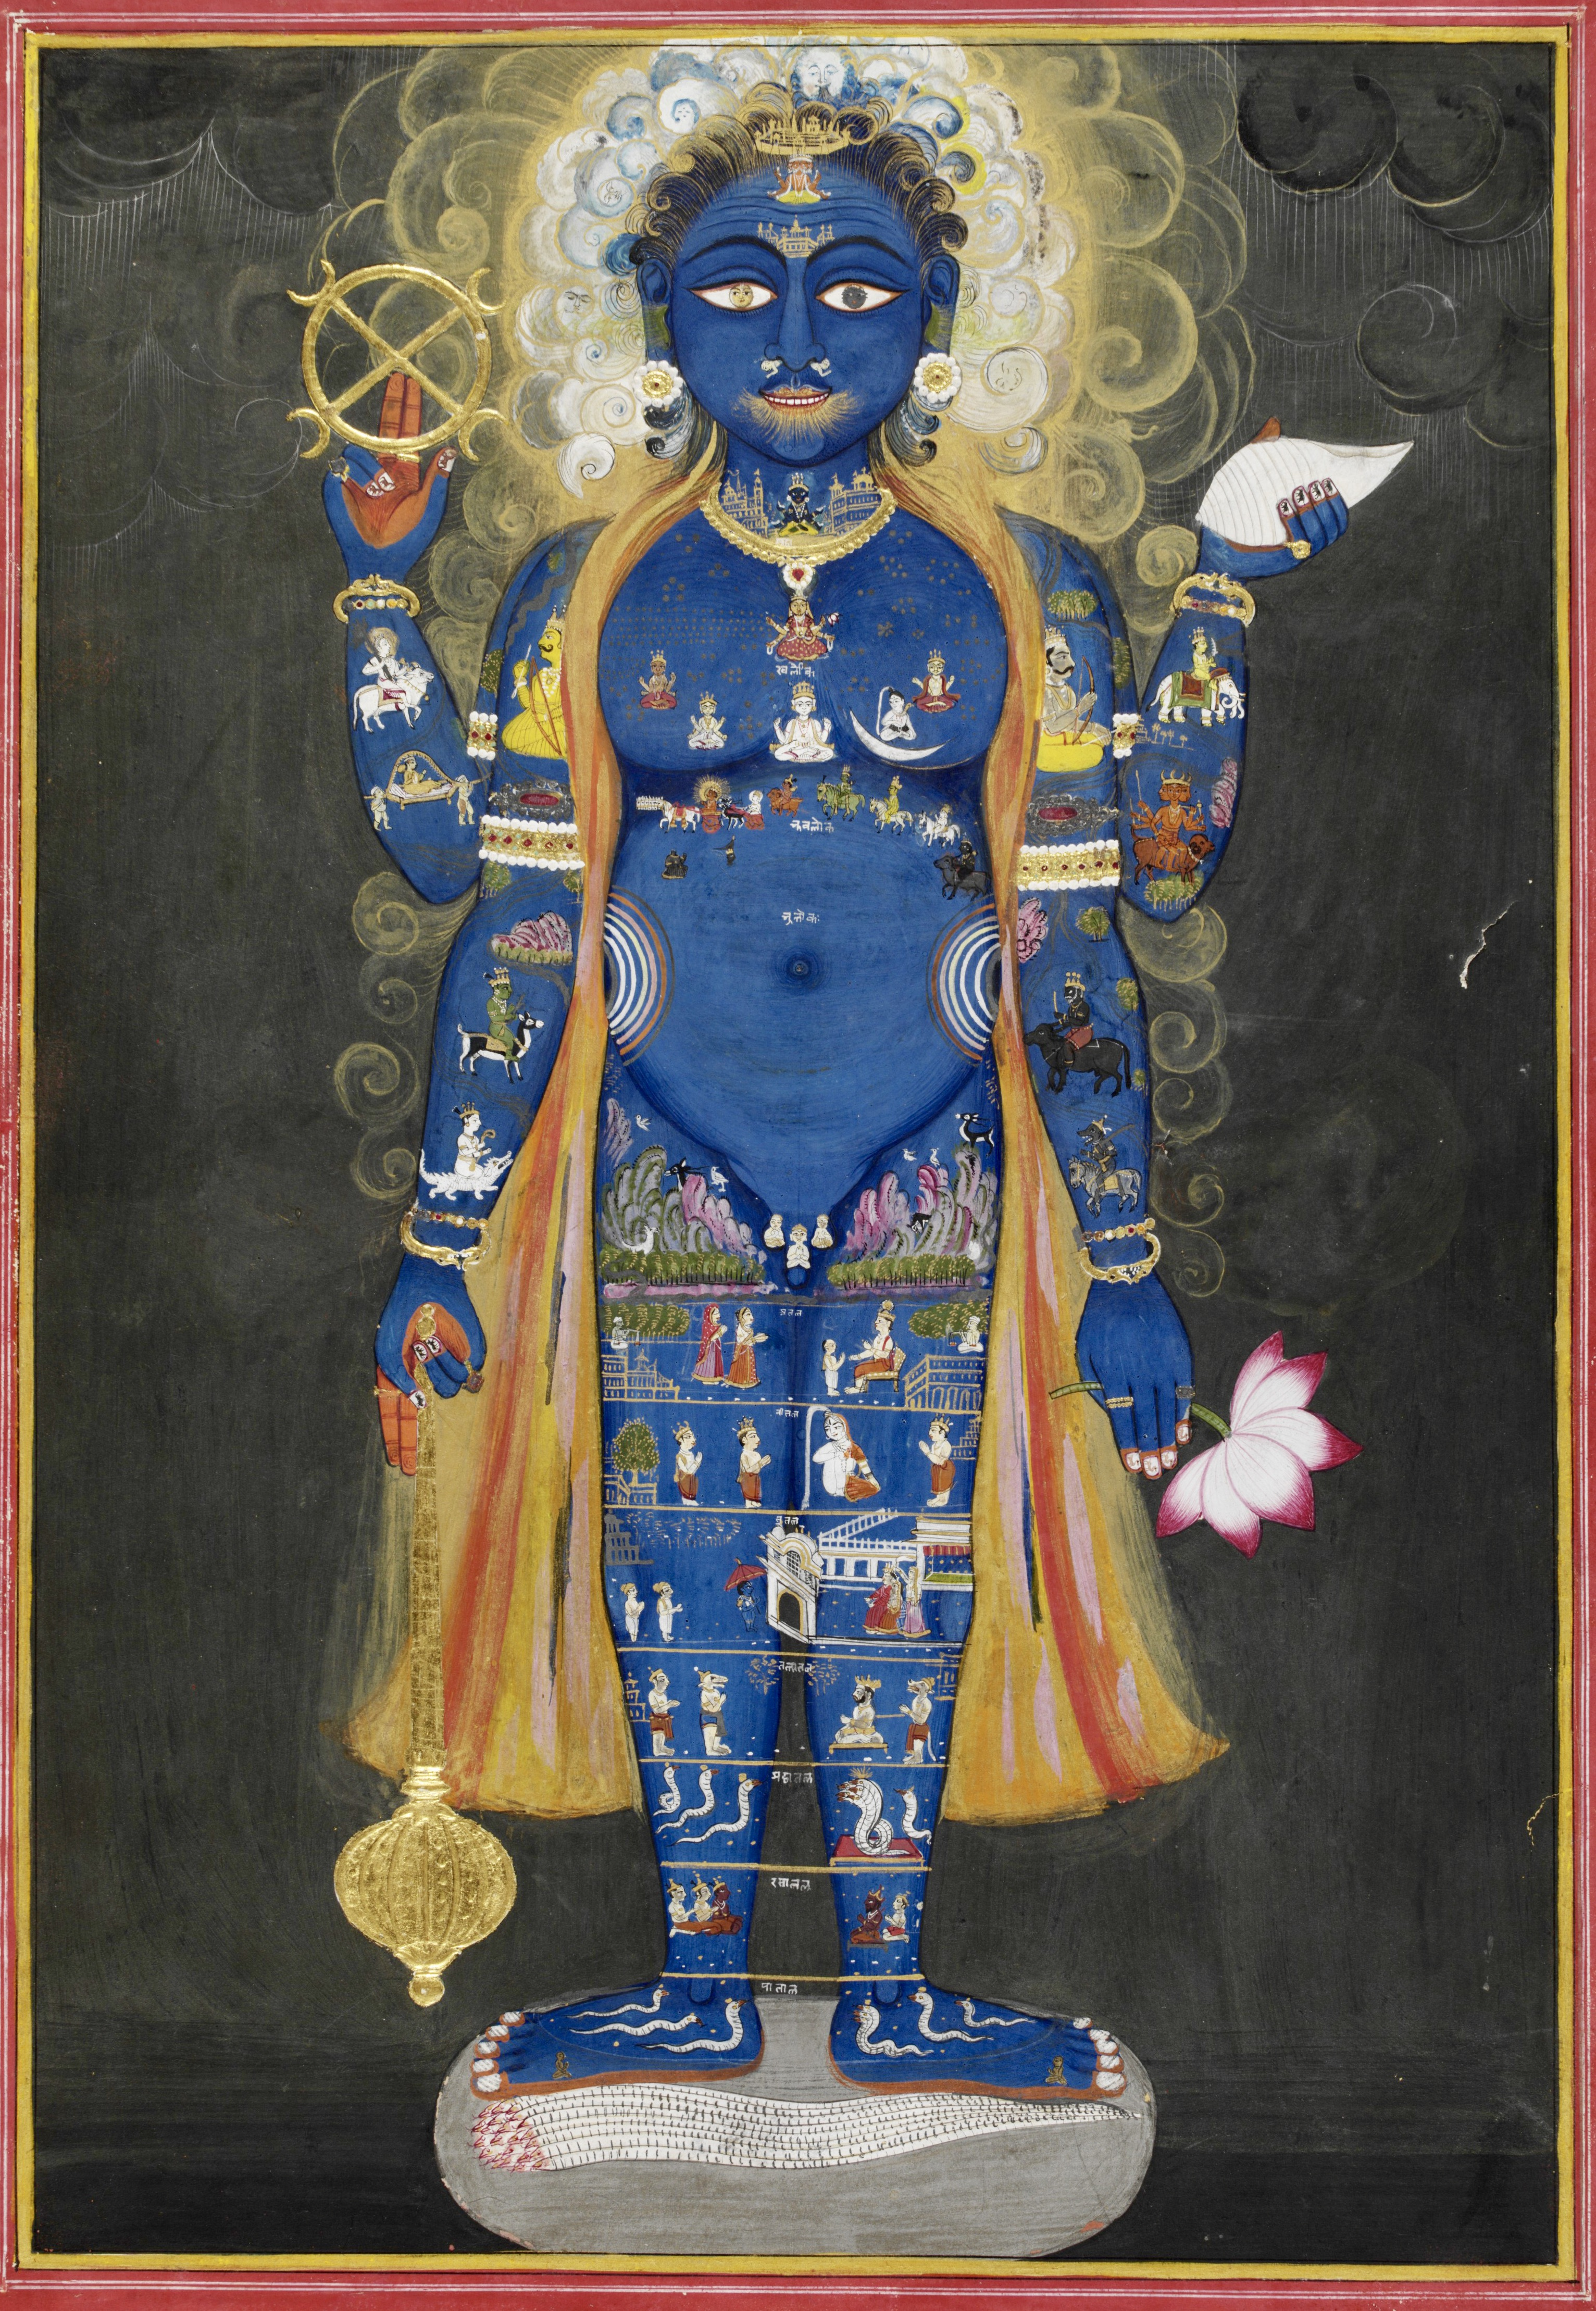
\includegraphics[width=1\textwidth]{pics/Vishnu_Vishvarupa_cropped.jpg}
	\caption{Viṣṇu Viśvarūpa, India, Rajasthan, Jaipur, ca. 1800–1820, Opaque watercolor and gold on paper, 38.5 × 28 cm, Victoria and Albert Museum, London, Given by Mrs. Gerald Clark.}
	\label{fig1}
      \end{figure}
\clearpage
  \begin{figure}[ht]
	\centering
  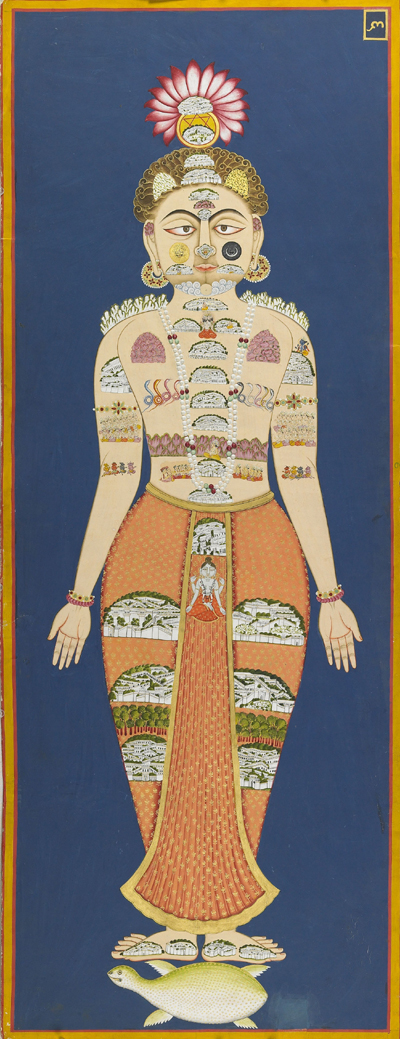
\includegraphics[width=0.5\textwidth]{pics/The_Equivalence_of_Self_and_Universe_(detail),_folio_6_from_the_Siddha_Siddhanta_Paddhati,_(Bulaki),_1824_(Samvat_1881);_122_x_46_cm._Mehrangarh_Museum_Trust..jpg}
	\caption{The Equivalence of Self and Universe (detail), folio 6 from the \textit{Siddhasiddhāntapaddhati} (Bulaki), India, Rajasthan, Jodhpur, 1824 (Samvat 1881), 122 x 46 cm, RJS 2378, Mehragarh Museum Trust.}
	\label{fig2}
      \end{figure}
      % \end{landscape}


\chapter{Bibliography}
 \label{sec:bibli}
   \clearpage
\newpage 
\thispagestyle{empty}
\quad  \addtocounter{page}{-1}

\printbibliography[heading=subbibintoc, title=Consulted Manuscripts, keyword=codex]

\printbibliography[heading=subbibintoc, title=Printed Editions, keyword=printsource]

\printbibliography[heading=subbibintoc, title=Secondary Literature, keyword=seclit]

\printbibliography[heading=subbibintoc, title=Online Sources, keyword=onlinesource]

\end{document}
